\chapter{Introducción al Análisis Dinámico}\label{cap4DIN}

En capítulos anteriores se cubrió el análisis de estructuras en régimen no lineal bajo la hipótesis de una respuesta estática. Un gran número de problemas prácticos requieren la capacidad de realizar análisis dinámicos de estructuras, se enumeran algunos a modo de ejemplo:
%
\begin{itemize}
	\item puentes y estructuras sometidas a cargas de tránsito dinámicas de tipo peatonal, carretero, ferroviario u otro,
	\item estructuras de soporte y/o fundaciones para maquinaria recíprocante o vibratoria,
	\item estructuras sometidas a movimientos sísmicos,
	\item impactos sobre estructuras,
	\item estructuras sometidas a explosiones.
\end{itemize}
%
Surge por lo tanto la necesidad de abandonar la hipótesis de carga estática y considerar el análisis dinámico de estructuras en régimen no lineal.

En este capítulo no se intenta cubrir el contenido de un curso de dinámica estructural, por el contrario, se busca únicamente sentar las bases de la resolución de problemas de dinámica no lineal, con lo cual, se omitirán conocimientos básicos de dinámica. %
%
Un libro recomendable para repasar dichos conocimientos básicos es \citep{clough1993dynamics}. %
%
La presentación que aquí se realiza está basada en los capítulos 9 y 24 de los libros \citep{Bathe2014} y \citep{Crisfield1997} respectivamente.

El presente capítulo consta a grandes rasgos de tres secciones. La primera presenta el planteo de las ecuaciones de movimiento de la estructura y describe sus componentes. La segunda sección presenta métodos de análisis dinámico y ejemplos para estructuras en régimen lineal. Finalmente, la tercera sección refiere a procedimientos de solución y ejemplos de estructuras no lineales.

\section{Deducción de las Ecuaciones de Movimiento}\label{EcMov}

Continuando con el material presentado en el Capítulo 2, se plantea a continuación la condición de equilibrio dinámico de una estructura compuesta por barras axiales con grandes desplazamientos y rotaciones pero pequeñas deformaciones unitarias.

En este contexto, se recurre al Principio de D'Alambert para establecer las ecuaciones de movimiento de un elemento de barra axial. Dicho principio es el equivalente dinámico al PTV. El mismo incorpora las fuerzas inerciales como fuerzas externas y permite expresar el equilibrio dinámico en forma variacional equivalente al PTV.

En lo que sigue, se hace referencia al tiempo mediante la variable independiente $t$ y se definen todas las variables estructurales (posición, desplazamiento, deformación unitaria, tensión, etc) como función del tiempo ($\bfx_t$, $\bfu_t$, $\sigma_t$, etc). %
%
Se utilizará la siguiente notación para expresar derivadas primera y segunda respecto del tiempo: $\dot{\bfu}_t$ y $\ddot{\bfu}_t$.

Dado lo anterior, para una barra axial, el Principio de D'Alambert sostiene que $\forall t$ y $\forall \delta \bfu \in \mcV$ se cumple:
%
\begin{equation}\label{DALAMBERT}
	\int_{V_t} \sigma_t \delta \varepsilon \dif V_t 
	= \int_{V_t}  \delta \bfu^\text{T} \bfb_{\text{ext},t} \, \dif V_t  - \int_{V_t} \rho_t \delta \bfu^\text{T} \ddot{\bfu}_t  \dif V_t - \int_{V_t} c \delta \bfu^\text{T} \dot{\bfu}_t  \dif V_t,
\end{equation}
%
donde $\bfb_{ext,t}$ representa el campo vectorial de fuerzas externas de volumen. %
%
Notar que, en la Ecuación~\eqref{DALAMBERT}, los vectores de desplazamiento $\bfu_t$ pertenecen a $\bbR^3$ que representan desplazamentos de partículas y no desplazamientos nodales.
 
En la Ecuación~\eqref{DALAMBERT}, la primer integral del miembro derecho corresponde a las fuerzas inerciales, siendo $\rho$ la densidad del material. Por otro lado, la segunda integral del miembro derecho corresponde a fuerzas viscosas disipativas, siendo $c>0$ un factor de disipación arbitrario.


La disipación viscosa presentada en este contexto es un mecanismo artificial para introducir efectos de amortiguamiento estructural. %
%
La misma no tiene, en general, un significado físico directo y por ende la disipación no se determinará usando una expresión teórica para $c$, sino que se realizará por medios empíricos. %
% -----------------

Aplicando una discretización de elementos finitos como la utilizada en el Capítulo 2 en la Ecuación~\eqref{DALAMBERT} y mediante consideraciones ya discutidas sobre el volumen de la barra para pequeñas deformaciones unitarias, se llega a la siguiente ecuación de movimiento a nivel de estructura:
%
\begin{equation}\label{EcMovNL}
	\bff_{\text{int}}(\bfu_t) = \bff_{\text{ext},t} - \bfM \ddot{\bfu}_t - \bfC \dot{\bfu}_t.
\end{equation}

Las cargas dinámicas externas están dadas por el vector $\bff_{\text{ext},t}$ y pueden ser periódicas (harmónicas, no harmónicas) o aperiódicas (impulsivas, transitorias). %
%
El tipo de carga influye en la definición del modelo estructural y a su vez en el método de resolución de las ecuaciones de movimiento resultantes.

El vector de fuerzas internas $\bff_{\text{int}}$ incorpora los efectos de no linealidad geométrica y eventualmente otros tipos de comportamiento no lineal de los elementos de barra, como puede ser la no linealidad material.

La matriz $\bfM$ es llamada Matriz de Masa. %
%
Si ésta se deduce usando las funciones de interpolación de $\bfu$ en la formulación de elementos finitos, se le suele llamar Matriz de Masa Consistente. Por el contrario, si es deducida concentrando la masa del elemento en sus nodos y asignándola a sus respectivos grados de libertad de desplazamiento, se la llama Matriz de Masa Concentrada. %
%
En este documento se consideran matrices de masa concentrada. %
%
Se puede verificar que los resultados obtenidos usando una u otra matriz son prácticamente equivalentes con una discretización suficientemente fina de elementos.

A modo de ejemplo se presenta la matriz de masa concentrada para el elemento de barra bi-dimensional:
%
\begin{equation}
\bfM^e = \frac{\rho A \ell_0}{2}
\left[\begin{matrix}
1 & 0 & 0 & 0\\
0 & 1 &0 & 0\\
0 & 0& 1 & 0\\
0 & 0 &0 & 1\\
\end{matrix}
\right]
\end{equation}

La matriz $\bfC$ es llamada Matriz de Amortiguamiento y permite incorporar los efectos disipativos viscosos de la estructura. %
%
Tal como fue indicado anteriormente, es habitual elegir una matriz $\bfC$ tal que de la aplicación de dicha matriz se obtengan amortiguamientos cercanos a valores empíricos conocidos para estructuras similares a la considerada. %
%
Por ejemplo, si se estudia una estructura metálica soldada y se sabe que una estructura de fabricación similar exhibió un cierto porcentaje del amortiguamiento crítico bajo vibraciones a ciertas frecuencias, se intentará elegir una matriz $\bfC$ que reproduzca esas características de amortiguamiento.

Una formulación usual para la matriz $\bfC$ es un tipo de amortiguamiento proporcional conocido como amortiguamiento de Rayleigh, ver \citep{clough1993dynamics}:
%
\begin{equation}
	\bfC = \eta \bfM + \chi \bfK.
\end{equation}

Esta matriz de amortiguamiento permite fijar valores aproximados de amortiguamiento para ciertos rangos de frecuencias y tiene la ventaja de ser esparza, al igual que $\bfK$. %
%
Es claro que otros tipos de amortiguamiento pueden ser incorporados mediante la matriz $\bfC$, por ejemplo amortiguadores conectados a dos nodos dados de la estructura. %
%
En estas situaciones se puede perder la característica de amortiguamiento proporcional.


\section{Dinámica Lineal}\label{DinLin}

Tal como fue mencionado, previo al abordaje de conceptos de dinámica no lineal, se presentará el problema y métodos de análisis de dinámica lineal. %
%

En esta sección se introducen dos métodos de integración directa de las ecuaciones de movimiento de uso habitual en la práctica. %
%
El primero de ellos es un método explícito, condicionalmente estable, llamado Método de Diferencia Centrada y el segundo es un método implícito, incondicionalmente estable bajo ciertas hipótesis, llamado Método de Newmark.


Antes de introducir los métodos, es conveniente escribir la ecuación de movimiento (ver Ecuación~\eqref{EcMovNL}) en la hipótesis de comportamiento lineal. %
%
Para ello, se asumen pequeñas deformaciones y desplazamientos y comportamiento material elástico lineal, de lo cual resulta una matriz de rigidez lineal $\bfK$ a nivel de estructura como la vista en cursos de elementos finitos lineales. %
%
En el caso de los elementos de barra vistos en el Capítulo 2, la matriz lineal del elemento corresponde a $\bfK^e=E A_0 \ell_0 \bfb_1^\text{T} \bfb_1$. %
%
Sea $\alpha$ el ángulo que forma la barra con la horizontal y llamando $c=\cos(\alpha)$ y $s=\sin(\alpha)$, se obtiene:
%
\begin{equation}
\bfK^e = \frac{E A}{\ell_0}
\left[\begin{matrix}
c^2 & c s & -c^2 & -c s\\
c s & s^2 & -c s & -s^2\\
-c^2 & -c s & c^2 & c s\\
-c s & -s^2 & c s & s^2\\
\end{matrix}
\right].
\end{equation}

Dado lo anterior, el vector de fuerzas internas $\bff_{\text{int}}(\bfu_t)$ está dado por $\bfK \bfu_t$, por lo que la ecuación de movimiento para el análisis dinámico lineal de la estructura resulta:
%
\begin{equation}\label{EcMovLin}
	\bfM \ddot{\bfu}_t + \bfC \dot{\bfu}_t + \bfK \bfu_t = \bff_{\text{ext},t}
\end{equation}

La Ecuación~\eqref{EcMovLin} representa un sistema de ecuaciones diferenciales ordinarias de segundo grado, con coeficientes constantes y no homogéneas. Para determinar una solución, se deben dar condiciones iniciales en el instante $t_0$ de desplazamiento ($\bfu_{t_0}$) y velocidad ($\dot{\bfu}_{t_0}$).

Las definiciones de las matrices $\bfM$ y $\bfC$, junto con comentarios generales sobre las mismas, ya fueron presentadas en la sección anterior y mantienen su validez.


\subsection{Método de Diferencia Centrada - Explícito}

El Método de Diferencia Centrada, presentado en esta sección, es probablemente el más sencillo entre los métodos de integración directa de las ecuaciones de movimiento. %
%
Por otra parte, este método puede resultar computacionalmente muy económico para ciertos modelos de elementos finitos y tipos de cargas dinámicas. 


Se verá más adelante que el método solamente requiere conocer la solución de la ecuación de movimiento en un instante de tiempo dado $t$ para poder determinar, mediante la evaluación de una expresión explícita, la solución en un tiempo posterior $t+\Delta t$. %
%
Esta característica es la que define a la clase de métodos \textit{explícitos}. %
%
Estos métodos son especialmente adecuados para resolver problemas dinámicos con transitorios rápidos, como ser el análisis de estructuras sometidas a impacto, explosiones o propagación de ondas.

A modo de ejemplo, el software \textit{Abaqus Explicit} utiliza este método de solución y permite modelar problemas del tipo indicado en el párrafo anterior\footnote{ver sitio web de \textit{Dassault Systèmes}\textsuperscript{\textregistered}.}. %
%
La formulación es levemente distinta a la presentada aquí, pero el método es el mismo.

\subsubsection{Formulación y Pseudo-código}

La formulación del método se basa en utilizar las siguientes aproximaciones de las derivadas de los desplazamientos, las cuales están basadas en diferencias centradas. Estas aproximaciones corresponden a las velocidades
%
\begin{equation}\label{DifCenVel}
\dot{\bfu}_t \simeq \frac{\bfu_{t+\Delta t}-\bfu_{t-\Delta t}}{2\Delta t},
\end{equation}
y aceleraciones
\begin{equation}\label{DifCenAccel}
	\ddot{\bfu}_t \simeq \frac{\bfu_{t+\Delta t}-2\bfu_{t}+\bfu_{t-\Delta t}}{\Delta t ^2}.
\end{equation}

Se asume que se conoce la solución hasta el instante $t$ y que, dado un incremento en el tiempo $\Delta t$, se desea hallar la solución en el instante $t+\Delta t$. %
%
Con lo cual, la incógnita a determinar es $\bfu_{t+\Delta t}$.

Para completar la definición del método, se debe utilizar la ecuación de movimiento. %
%
En particular, se considera el equilibrio dinámico en el instante $t$, dado por la Ecuación~\eqref{EcMovLin} y se sustituyen las expresiones aproximadas para la aceleración y la velocidad, dadas por las Ecuaciones \eqref{DifCenAccel} y \eqref{DifCenVel}. %
%
Realizando esto se obtiene:
%
\begin{equation}
\bfM \left[\frac{\bfu_{t+\Delta t}-2\bfu_{t}+\bfu_{t-\Delta t}}{\Delta t ^2}\right] + \bfC \left[\frac{\bfu_{t+\Delta t}-\bfu_{t-\Delta t}}{2\Delta t}\right] + \bfK \bfu_t = \bff_{\text{ext},t}.
\end{equation}

Despejando el desplazamiento incógnita $\bfu_{t+\Delta t}$ se llega a que:
%
\begin{equation}\label{EcDifCent}
\begin{split}
	\left[\frac{1}{\Delta t^2}\bfM + \frac{1}{2\Delta t}\bfC \right] \bfu_{t+\Delta t} = \bff_{\text{ext},t} - & \left[\bfK-\frac{2}{\Delta t ^2}\bfM\right] \bfu_t \\
	-& \left[\frac{1}{\Delta t^2}\bfM-\frac{1}{2\Delta t}\bfC\right] \bfu_{t-\Delta t}
\end{split}
\end{equation}

Notar que en este método se aproximan las aceleraciones y velocidades en el instante $t$, este error suele llamarse error de truncamiento en referencia al truncamiento de una serie de Taylor. %
%
Cabe observar que este error de truncamiento puede ser reducido eligiendo un paso temporal $\Delta t$ más pequeño. %
%
En segundo lugar, se introduce otro error al determinar la solución en el tiempo $t+\Delta t$ a partir del equilibrio dinámico en el instante $t$. Es inmediato ver que las aceleraciones, velocidades y desplazamientos del tiempo $t+\Delta t$ hallados mediante este método no satisfarán exactamente la ecuación de movimiento en el tiempo $t + \Delta t$.

En el Algoritmo~\ref{PCDifCent} se presenta un Pseudo-Código del método.

\begin{algorithm}[htb]
\caption{Método de Diferencia Centrada.} \label{PCDifCent}
	\begin{algorithmic}[1]
	\STATE Ensamblar: $\bfM$, $\bfK$ y $\bfC$ a nivel de estructura.
	\STATE Definir: tiempo final de análisis dinámico: $t_f$
	\STATE Definir: Condiciones iniciales: $\bfu_{0}$, $\dot{\bfu}_{0}$
	\STATE Calcular: $\ddot{\bfu}_{0}\leftarrow \bfM^{-1}(\bff_{ext,t} - \bfC \dot{\bfu}_0 - \bfK \bfu_0)$
	\STATE Definir: $\Delta t$ tal que $\Delta t < T_{min} / \pi$
	\STATE Calcular: $a_0\leftarrow1/\Delta t^2$, $a_1\leftarrow1/(2\Delta t)$, $a_2\leftarrow2a_0$ y $a_3\leftarrow1/a_2$
	\STATE Calcular: $\bfu_{-\Delta t} \leftarrow \bfu_0 - \Delta t \dot{\bfu}_0 + a_3\ddot{\bfu}_0$
	\STATE Calcular y factorizar: $\hat{\bfM}\leftarrow a_0\bfM+a_1\bfC$
	\STATE $t \leftarrow 0$
	\WHILE{$t<t_f$}
		\STATE Calcular: $\hat{\bff}_t\leftarrow \bff_{ext,t} - (\bfK-a_2\bfM)\bfu_t - (a_0\bfM-a_1\bfC)\bfu_{t-\Delta t}$
		\STATE Resolver: $\bfu_{t+\Delta t}\leftarrow \hat{\bfM}^{-1}\hat{\bff}_t$
		\STATE Calcular aceleración: $\ddot{\bfu}_{t}\leftarrow a_0(\bfu_{t+\Delta t}-2\bfu_{t}+\bfu_{t-\Delta t})$
		\STATE Calcular velocidad: $\dot{\bfu}_{t}\leftarrow a_1(\bfu_{t+\Delta t}-\bfu_{t-\Delta t})$
		\STATE $t\leftarrow t+\Delta t$
	\ENDWHILE	
\end{algorithmic}
\end{algorithm}

Analizando la línea 12 del Pseudo-Código se puede ver que este método puede ser extremadamente económico desde el punto de vista computacional si la matriz $\hat{\bfM}$ es invertible de manera económica, particularmente si esta matriz es diagonal. %
%
Es por esto que al aplicar este método se utiliza la matriz de Masa Concentrada y no la matriz de Masa Consistente. %
%
Adicionalmente, la matriz de efectos viscosos puede ser despreciada en fenómenos rápidos de muy corta duración. %
%
En su defecto, se utiliza una matriz $\bfC$ diagonal de manera de no aumentar el costo computacional.


\subsubsection{Estabilidad Numérica}\label{DifCenStab}

En el Algoritmo~\ref{PCDifCent} se indica que el valor del paso temporal elegido debe satisfacer la condición: $\Delta t < T_{min}/\pi$, donde $T_{min}$ es el mínimo período de vibración natural del modelo de elementos finitos. Para entender esta restricción, se realiza el análisis de la estabilidad numérica del Método de Diferencia Centrada.

El análisis de estabilidad numérica se lleva a cabo en una estructura sin amortiguamiento, es decir con $\bfC = 0$. Sin embargo, es posible analizar la estabilidad tomando en cuenta el amortiguamiento, en particular bajo la hipótesis de amortiguamiento proporcional. %
%
Se realizará algún comentario adicional a este punto más adelante en esta sección.

Previo a realizar el análisis de estabilidad numérica, se debe reconocer que es suficiente estudiar la estabilidad de la solución numérica de un sistema con un grado de libertad. %
%
La justificación de este hecho se basa en la descomposición modal de la respuesta de la estructura y se describe brevemente a continuación.

Se definen los modos normales de vibración de la estructura como aquellas soluciones de vibración libre no forzada en las que todos los puntos de la estructura se desplazan de forma sinusoidal respecto del tiempo, en fase y a una misma frecuencia; es decir: $\bfu_t = \sin(\omega(t-t_0)) \bfphi $, donde $\bfphi$ es un vector de desplazamientos nodales asociados a las amplitudes del movimiento.

Sustituyendo el modo normal definido anteriormente en la ecuación de movimiento (sin amortiguamiento ni fuerzas externas) se obtiene la siguiente relación:
%
\begin{equation}
	\omega^2 \bfM \bfphi = \bfK \bfphi.
\end{equation}

La ecuación anterior define un problema de valores propios para una matriz simétrica definida positiva. Esto implica que existen tantos modos normales \{$\bfphi_i$ , $\omega_i^2$\} como grados de libertad tenga la estructura ($n$), es decir tantos como la dimensión de las matrices $\bfM$ o $\bfK$ (reducidas). %

\cajaactividad{Mostrar que los modos normales de vibración satisfacen la relación:
	$$\bfphi_i^T\bfM \bfphi_j = \delta_{ij} \quad i,j=1,\dots,n,
	$$
	donde $\delta_{ij}$ es el delta de Kronecker.}

Agrupando cada uno de los $n$ modos normales $\bfphi_i$ como columnas de una matriz $\bfPhi$, y sus respectivas frecuencias al cuadrado ($\omega_i^2$) en la diagonal de una matriz $\bfLam$, se tiene:
%
\begin{equation}\label{ModosNormales}
\bfM \bfPhi \bfLam = \bfK \bfPhi
\end{equation}

La Ecuación~\eqref{ModosNormales} define la relación matricial que verifican los modos normales de la estructura. Queda definida así una base de vectores dada por $\bfPhi$ en la cual se pueden escribir los vectores de desplazamiento a lo largo del tiempo.

A partir del desarrollo anterior, se define $\bfu_t = \bfPhi \bfx_t$. Es decir, $\bfx_t$ son las coordenadas que representan a $\bfu_t$ en la base de modos normales $\bfPhi$. La ecuación de movimiento resulta:
%
\begin{equation}\label{EcMovDiag1}
	\bfM \bfPhi \ddot{\bfx}_t + \bfK \bfPhi \bfx_t = \bff_{\text{ext},t}.
\end{equation}

Si se multiplica la Ecuación~\eqref{EcMovDiag1} a la izquierda por $\bfPhi^T$ se obtiene,
%
\begin{equation}\label{EcMovDiag2}
\bfPhi^T \bfM \bfPhi \ddot{\bfx}_t + \bfPhi^T \bfK \bfPhi \bfx_t = \bfPhi^T \bff_{\text{ext},t}.
\end{equation}
%
Usando la condición de $\bfM$-ortonormalidad de los vectores $\bfphi_i$ y definiendo $\bfnu_t=\bfPhi^T \bff_{\text{ext},t}$ se llega a:
%
\begin{equation}\label{EcMovDiag}
\ddot{\bfx}_t + \bfLam \bfx_t = \bfnu_t.
\end{equation}

De la Ecuación~\eqref{EcMovDiag} se puede concluir que al cambiar la base a $\bfPhi$, la ecuación de movimiento queda diagonalizada o en otras palabras se desacoplan las ecuaciones de movimiento de los distintos grados de libertad. En la nueva base se tiene:
%
\begin{equation}
\ddot{x}_{i,t} + \omega^2_i x_{i,t} = \nu_{i,t} \quad  i=1...n.
\end{equation}

Un breve comentario respecto del amortiguamiento. Si se considera el amortiguamiento, el argumento anterior es válido solamente si se asume que la matriz de amortiguamiento $\bfC$ cumple que $\bfPhi^T \bfC \bfPhi$ es una matriz diagonal. %
%
Queda como ejercicio verificar lo anterior. %
%
En esos casos se llega a ecuaciones de movimiento desacopladas de la forma:
%
\begin{equation}\label{EcMovDiagAmor}
\ddot{x}_{i,t} + 2\xi_i\omega_i \dot{x}_{i,t} + \omega^2_i x_{i,t} = \nu_{i,t}
\end{equation}

Queda establecido que se puede analizar el comportamiento de la solución numérica de la ecuación de movimiento de un sistema de un grado de libertad sin amortiguamiento y considerando varias componentes se abarca el análisis de una estructura completa.

Se define por lo tanto el \textit{Problema Test} con el cual se analiza la estabilidad numérica del Método de Diferencia Centrada:
%
\begin{equation}\label{Ptest}
\text{Problema Test}
\begin{cases} 
\ddot{x}_t + \omega^2 x_t = 0\\
x_0 = 1 \\
\dot{x}_0 = 0\\
\end{cases}
\end{equation}

La aplicación del método de Diferencia Centrada al Problema Test resulta en la siguiente ecuación,
%
\begin{equation}\label{DifCent1DOF}
	x_{t+\Delta t} = (2-\omega_i^2 \Delta t^2)x_t - x_{t-\Delta t}.
\end{equation}

Se define el vector $\hat{\bfx}_{t+\Delta t} = [x_{t+\Delta t}, x_t]^T$. Usando la Ecuación~\eqref{DifCent1DOF} se puede presentar la solución con el método de Diferencia Centrada de la siguiente forma,
%
\begin{equation}\label{DifCentMatricial}
\hat{\bfx}_{t+\Delta t} = \bfA \hat{\bfx}_{t},
\end{equation}
donde la matriz $\bfA$ está definida como,
%
\begin{equation}\label{MatrizA}
\bfA = \left[\begin{matrix}
2-\omega_i^2 \Delta t^2 & -1 \\
1 & 0 \\
\end{matrix}
\right].
\end{equation}

El vector $\hat{\bfx}_{0}$ es un vector constante, no nulo, que queda definido a partir de las condiciones iniciales del Problema Test. %
%
Se puede suponer sin perder generalidad que $t=n \Delta t$ con $n\in \mathbb{N}$. Por lo tanto, la aplicación repetida de la Ecuación~\eqref{DifCentMatricial} permite obtener:
%
\begin{equation}\label{DifCentMatricial2}
\hat{\bfx}_{t} = \bfA^n \hat{\bfx}_{0}
\end{equation}

Es aquí que se impone el criterio de estabilidad numérica. Un sistema de un grado de libertad, sin amortiguamiento y sin forzamiento externo, que parte de una condición inicial dada tiene una solución oscilatoria que permanece acotada. Es natural por lo tanto, requerir que la solución numérica no diverja. Es decir que para todo instante $t$ se cumpla $\|\hat{\bfx}_t\|<\infty$.

Tomando normas en la Ecuación~\eqref{DifCentMatricial2} se obtiene la identidad:
%
\begin{equation}\label{MIM}
\|\hat{\bfx}_{t}\| = \|\bfA^n \hat{\bfx}_{0}\|.
\end{equation}

El miembro derecho de la Ecuación~\eqref{MIM} está acotado si, se cumple que el radio espectral de $\bfA$ es menor a 1, es decir $\rho(\bfA)<1$. %
%
El radio espectral de $\bfA$ se define como el máximo de los módulos de los valores propios de la matriz $\bfA$, es decir: $\rho(\bfA)=\max_i |\lambda_i|$. Si la multiplicidad de los valores propios es uno, la condición se puede relajar a $\rho(\bfA)\leq 1$.

La justificación formal de este punto se puede buscar en las notas del curso \textit{Métodos Numéricos} (Facultad de Ingeniería, \textit{Universidad de la República}). %
%
Alternativamente, un idea intuitiva de la validez de este resultado puede obtenerse pensando en que si $\bfA$ es diagonalizable ($\bfA = \bfP^{-1}\bfD \bfP$), entonces $\bfA^n = \bfP^{-1} \bfD^n \bfP$. Si los módulos de todos los valores propios que hay en la diagonal de $\bfD$ son menores a 1, se tiene que $\bfD^n\rightarrow 0$.

Por lo tanto, para evaluar la condición de estabilidad del método en cuestión debemos calcular los valores propios de $\bfA$, verificar que tienen multiplicidad igual a uno, e imponer que el módulo de éstos sea menor o igual a 1. 

Se define $z=\omega \Delta t>0$ con lo cual los valores propios resultan:
%
\begin{equation}\label{VProps}
\lambda_{1,2} = \frac{2-z^2}{2}\pm\sqrt{\frac{(2-z^2)^2}{4}-1}.
\end{equation}
%
Se puede ver que los valores propios tienen multiplicidad 1, incluso cuando $z=2$. %

En la Figura~\ref{fig:StabDifCentr} se presenta la gráfica de la función $\rho(\bfA)(z)=\max\{|\lambda_1(z)|,|\lambda_2(z)|\}$ para valores $z\in[0,3]$.

\begin{figure}[htb]
	\centering
	\resizebox{.58\linewidth}{!}{% Title: gl2ps_renderer figure
% Creator: GL2PS 1.4.0, (C) 1999-2017 C. Geuzaine
% For: Octave
% CreationDate: Sat May  8 08:49:58 2021
\setlength{\unitlength}{1pt}
\begin{picture}(0,0)
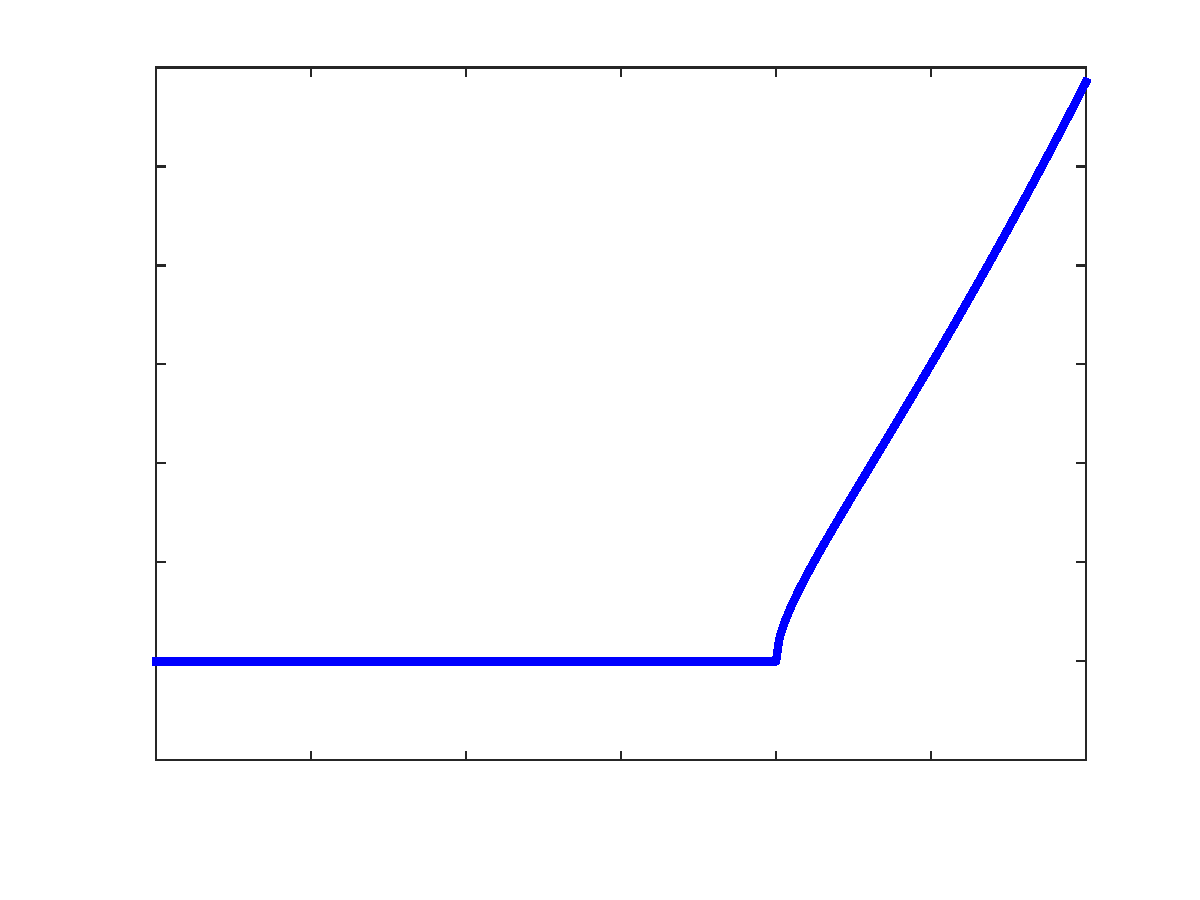
\includegraphics{Stabil-inc}
\end{picture}%
\begin{picture}(576,432)(0,0)
\fontsize{20}{0}
\selectfont\put(74.88,52){\makebox(0,0)[t]{\textcolor[rgb]{0.15,0.15,0.15}{{0}}}}
\fontsize{20}{0}
\selectfont\put(149.28,52){\makebox(0,0)[t]{\textcolor[rgb]{0.15,0.15,0.15}{{0.5}}}}
\fontsize{20}{0}
\selectfont\put(223.68,52){\makebox(0,0)[t]{\textcolor[rgb]{0.15,0.15,0.15}{{1}}}}
\fontsize{20}{0}
\selectfont\put(298.08,52){\makebox(0,0)[t]{\textcolor[rgb]{0.15,0.15,0.15}{{1.5}}}}
\fontsize{20}{0}
\selectfont\put(372.48,52){\makebox(0,0)[t]{\textcolor[rgb]{0.15,0.15,0.15}{{2}}}}
\fontsize{20}{0}
\selectfont\put(446.88,52){\makebox(0,0)[t]{\textcolor[rgb]{0.15,0.15,0.15}{{2.5}}}}
\fontsize{20}{0}
\selectfont\put(521.28,52){\makebox(0,0)[t]{\textcolor[rgb]{0.15,0.15,0.15}{{3}}}}
\fontsize{20}{0}
\selectfont\put(64.871,66.9828){\makebox(0,0)[r]{\textcolor[rgb]{0.15,0.15,0.15}{{0}}}}
\fontsize{20}{0}
\selectfont\put(64.871,114.499){\makebox(0,0)[r]{\textcolor[rgb]{0.15,0.15,0.15}{{1}}}}
\fontsize{20}{0}
\selectfont\put(64.871,162.016){\makebox(0,0)[r]{\textcolor[rgb]{0.15,0.15,0.15}{{2}}}}
\fontsize{20}{0}
\selectfont\put(64.871,209.533){\makebox(0,0)[r]{\textcolor[rgb]{0.15,0.15,0.15}{{3}}}}
\fontsize{20}{0}
\selectfont\put(64.871,257.05){\makebox(0,0)[r]{\textcolor[rgb]{0.15,0.15,0.15}{{4}}}}
\fontsize{20}{0}
\selectfont\put(64.871,304.566){\makebox(0,0)[r]{\textcolor[rgb]{0.15,0.15,0.15}{{5}}}}
\fontsize{20}{0}
\selectfont\put(64.871,352.083){\makebox(0,0)[r]{\textcolor[rgb]{0.15,0.15,0.15}{{6}}}}
\fontsize{20}{0}
\selectfont\put(64.871,399.6){\makebox(0,0)[r]{\textcolor[rgb]{0.15,0.15,0.15}{{7}}}}
\fontsize{22}{0}
\selectfont\put(298.08,32){\makebox(0,0)[t]{\textcolor[rgb]{0.15,0.15,0.15}{{$\omega_i \Delta t$}}}}
\fontsize{22}{0}
\selectfont\put(48.871,233.291){\rotatebox{90}{\makebox(0,0)[b]{\textcolor[rgb]{0.15,0.15,0.15}{{$\rho$}}}}}
\end{picture}
}
	\caption{Condición de Estabilidad del Método de Diferencia Centrada.}
	\label{fig:StabDifCentr}
\end{figure}

Se observa que se satisface el criterio de estabilidad si se cumple $\omega \Delta t \leq 2$. Llamando $T$ al período asociado a $\omega$, la condición es equivalente a: $\Delta t/ T \leq 1/\pi$.

En una estructura completa, todos los grados de libertad deben satisfacer esta condición. Se observa que la condición más estricta para $\Delta t$ corresponde al grado de libertad con el período natural más corto (es decir, el de mayor frecuencia), con lo cual el criterio de estabilidad numérica para una estructura completa es:
%
\begin{equation}
	\Delta t \leq \frac{T_{\text{min}}}{\pi},
\end{equation}
%
siendo $T_{\text{min}}$ el menor período natural.

\subsubsection{Ejemplo - Edificio Sometido a Carga de Explosión}\label{EjBlast}

Se considera la estructura de un edificio de hormigón armado con tres niveles, conformada por pilares, vigas y losas. %
%
La estructura considerada no representa una estructura realista, sino simplemente una idealización simplificada de un edificio. %

La geometría del edificio y la posición de la detonación considerada se muestra en la Figura~\ref{fig:Edificio} a través de una vista en planta (arriba) y un corte vertical (abajo).

\begin{figure}[htb]
	\centering
	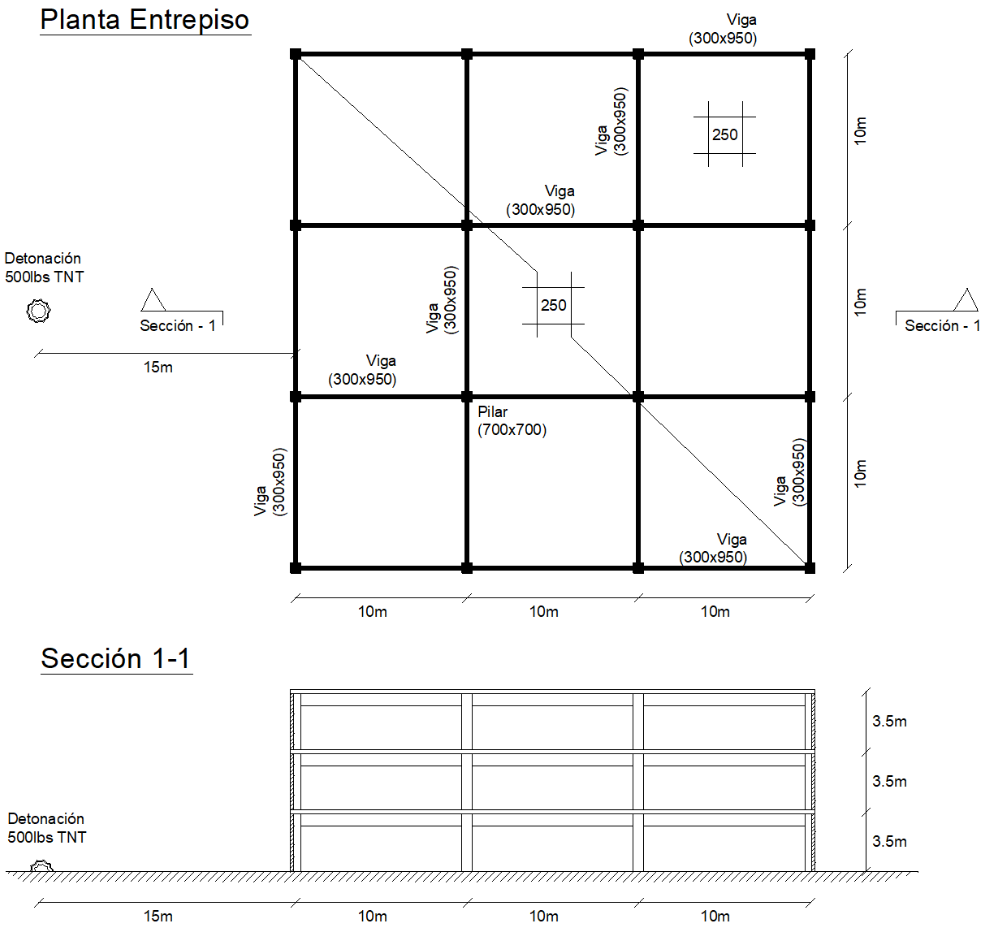
\includegraphics[width=.9\linewidth]{../fig/edificio}
	\caption{Esquema de la Estructura del Edificio.}
	\label{fig:Edificio}
\end{figure}


Se considera que los pilares se empotran significativamente en los entrepisos y que los entrepisos son rígidos (a flexión y directa) en el plano. %
%
Con lo cual el movimiento lateral de la estructura en una dirección queda completamente definida por el desplazamiento lateral de cada piso ($u_1,u_2,u_3$) respecto de la posición original vertical. %
%
Esto permite realizar una idealización de la estructura a través de un modelo unidimensional mostrado en la Figura~\ref{fig:3dof}.

\begin{figure}[htb]
	\centering
	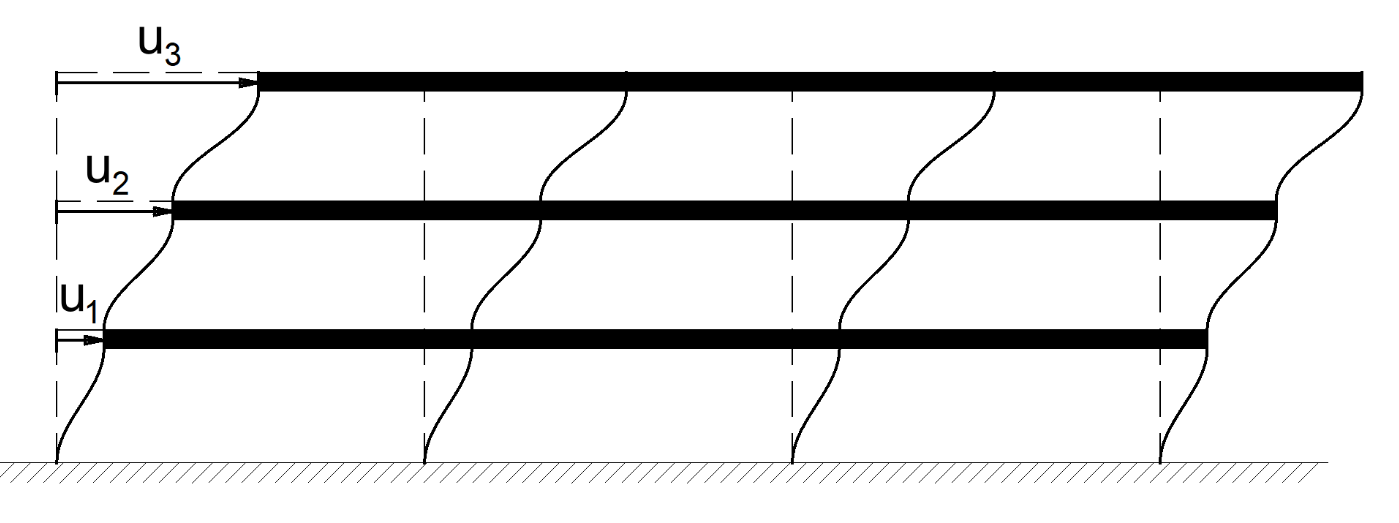
\includegraphics[width=.6\linewidth]{../fig/model3dof}
	\caption{Modelo del Edificio con 3 Grados de Libertad.}
	\label{fig:3dof}
\end{figure}

Dada la idealización estructural considerada, se plantea realizar el análisis dinámico lineal de la estructura. %
%
Se utiliza una matriz de masas concentradas, en la cual cada grado de libertad concentra la masa entre pisos adyacentes. Por otro lado, la matriz de rigidez se obtiene considerando la rigidez de un pilar empotrado-empotrado deslizante y la cantidad de pilares que se conectan a un entrepiso. Siendo $\bfu_t=[u_{1,t}, u_{2,t}, u_{3,t}]^T$,
%
\begin{equation}
\bfK = \frac{n_{cols} 12 E I }{H^3}
\left[\begin{matrix}
2 & -1 & 0 \\
-1 & 2 & -1 \\
0 & -1 & 1 \\
\end{matrix}
\right]
\end{equation}

La carga dinámica a la cual es sometido el edificio corresponde a las presiones generadas sobre la envolvente del edificio a causa de la detonación equivalente a 500 lbs de TNT a nivel de piso y a una distancia de 15m del edificio. Las presiones que se utilizan en el ejemplo fueron obtenidas del documento \citep{aisc2013guide26}.

Se resuelve la dinámica mediante el Método de Diferencia Centrada. La selección  del paso temporal $\Delta t$ se hizo considerando que se debía satisfacer la estabilidad numérica y que se debía capturar con suficiente precisión la súbita carga de presión de la explosión. %
%
El resultado del análisis numérico se muestra en la Figura~\ref{fig:blast}.

\begin{figure}[htb]
	\centering
	\resizebox{.97\linewidth}{!}{% Title: Figure 1
% Creator: GL2PS 1.4.2, (C) 1999-2020 C. Geuzaine
% For: Octave
% CreationDate: Mon Aug  5 15:53:53 2024
\setlength{\unitlength}{1pt}
\begin{picture}(0,0)
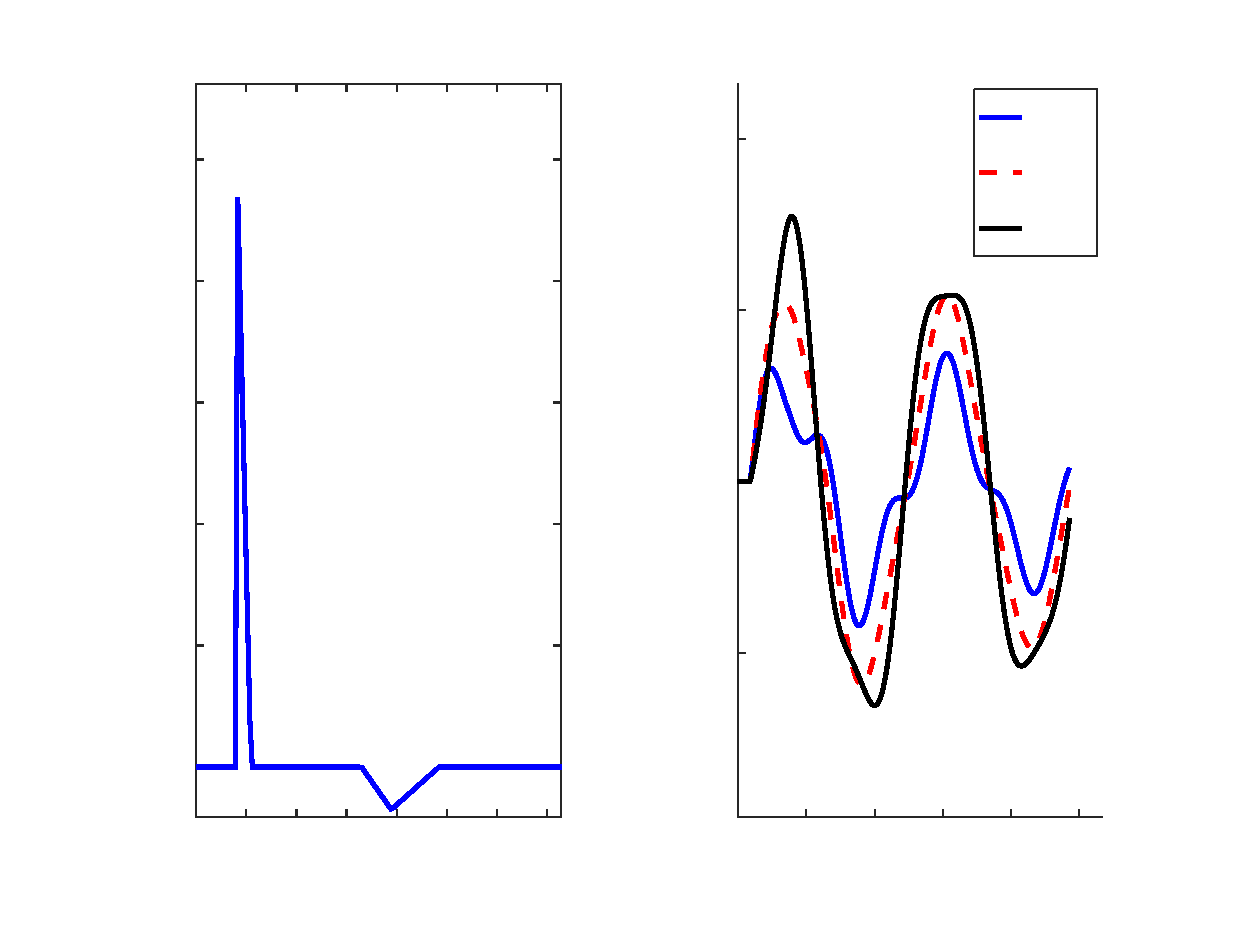
\includegraphics[scale=1]{Explicit-inc}
\end{picture}%
\begin{picture}(420,315)(0,0)
\fontsize{13}{0}\selectfont\put(54.6199,176.8){\makebox(0,0)[t]{\textcolor[rgb]{0.15,0.15,0.15}{{0}}}}
\fontsize{13}{0}\selectfont\put(115.55,176.8){\makebox(0,0)[t]{\textcolor[rgb]{0.15,0.15,0.15}{{0.1}}}}
\fontsize{13}{0}\selectfont\put(176.481,176.8){\makebox(0,0)[t]{\textcolor[rgb]{0.15,0.15,0.15}{{0.2}}}}
\fontsize{13}{0}\selectfont\put(237.412,176.8){\makebox(0,0)[t]{\textcolor[rgb]{0.15,0.15,0.15}{{0.3}}}}
\fontsize{13}{0}\selectfont\put(298.342,176.8){\makebox(0,0)[t]{\textcolor[rgb]{0.15,0.15,0.15}{{0.4}}}}
\fontsize{13}{0}\selectfont\put(359.273,176.8){\makebox(0,0)[t]{\textcolor[rgb]{0.15,0.15,0.15}{{0.5}}}}
\fontsize{13}{0}\selectfont\put(48.1275,193.717){\makebox(0,0)[r]{\textcolor[rgb]{0.15,0.15,0.15}{{0}}}}
\fontsize{13}{0}\selectfont\put(48.1275,211.074){\makebox(0,0)[r]{\textcolor[rgb]{0.15,0.15,0.15}{{100}}}}
\fontsize{13}{0}\selectfont\put(48.1275,228.431){\makebox(0,0)[r]{\textcolor[rgb]{0.15,0.15,0.15}{{200}}}}
\fontsize{13}{0}\selectfont\put(48.1275,245.788){\makebox(0,0)[r]{\textcolor[rgb]{0.15,0.15,0.15}{{300}}}}
\fontsize{13}{0}\selectfont\put(48.1275,263.146){\makebox(0,0)[r]{\textcolor[rgb]{0.15,0.15,0.15}{{400}}}}
\fontsize{13}{0}\selectfont\put(48.1275,280.503){\makebox(0,0)[r]{\textcolor[rgb]{0.15,0.15,0.15}{{500}}}}
\fontsize{14}{0}\selectfont\put(217.429,162.8){\makebox(0,0)[t]{\textcolor[rgb]{0.15,0.15,0.15}{{t [s]}}}}
\fontsize{14}{0}\selectfont\put(25.1275,238.92){\rotatebox{90}{\makebox(0,0)[b]{\textcolor[rgb]{0.15,0.15,0.15}{{presion [kPa]}}}}}
\fontsize{15}{0}\selectfont\put(66.4939,31.1353){\makebox(0,0)[t]{\textcolor[rgb]{0.15,0.15,0.15}{{0}}}}
\fontsize{15}{0}\selectfont\put(125.203,31.1353){\makebox(0,0)[t]{\textcolor[rgb]{0.15,0.15,0.15}{{0.1}}}}
\fontsize{15}{0}\selectfont\put(183.911,31.1353){\makebox(0,0)[t]{\textcolor[rgb]{0.15,0.15,0.15}{{0.2}}}}
\fontsize{15}{0}\selectfont\put(242.62,31.1353){\makebox(0,0)[t]{\textcolor[rgb]{0.15,0.15,0.15}{{0.3}}}}
\fontsize{15}{0}\selectfont\put(301.328,31.1353){\makebox(0,0)[t]{\textcolor[rgb]{0.15,0.15,0.15}{{0.4}}}}
\fontsize{15}{0}\selectfont\put(360.037,31.1353){\makebox(0,0)[t]{\textcolor[rgb]{0.15,0.15,0.15}{{0.5}}}}
\fontsize{15}{0}\selectfont\put(59,63.5394){\makebox(0,0)[r]{\textcolor[rgb]{0.15,0.15,0.15}{{-0.005}}}}
\fontsize{15}{0}\selectfont\put(59,85.6135){\makebox(0,0)[r]{\textcolor[rgb]{0.15,0.15,0.15}{{0}}}}
\fontsize{15}{0}\selectfont\put(59,107.688){\makebox(0,0)[r]{\textcolor[rgb]{0.15,0.15,0.15}{{0.005}}}}
\fontsize{15}{0}\selectfont\put(59,129.762){\makebox(0,0)[r]{\textcolor[rgb]{0.15,0.15,0.15}{{0.01}}}}
\fontsize{15}{0}\selectfont\put(223.366,15.1353){\makebox(0,0)[t]{\textcolor[rgb]{0.15,0.15,0.15}{{t [s]}}}}
\fontsize{15}{0}\selectfont\put(16,89.6158){\rotatebox{90}{\makebox(0,0)[b]{\textcolor[rgb]{0.15,0.15,0.15}{{desplazamiento [m]}}}}}
\fontsize{13}{0}\selectfont\put(342.243,118.306){\makebox(0,0)[l]{\textcolor[rgb]{0,0,0}{{$u_1$}}}}
\fontsize{13}{0}\selectfont\put(342.243,101.308){\makebox(0,0)[l]{\textcolor[rgb]{0,0,0}{{$u_2$}}}}
\fontsize{13}{0}\selectfont\put(342.243,84.3091){\makebox(0,0)[l]{\textcolor[rgb]{0,0,0}{{$u_3$}}}}
\end{picture}
}
	\caption{Solución numérica de dinámica de edificio sometido a carga de explosión: historia de presiones considerada (izquierda) y respuesta de la estructura (derecha).}
	\label{fig:blast}
\end{figure}

Se puede ver el período de reposo previo al impacto de la explosión, seguido por una respuesta dinámica gobernada por el modo fundamental con los otros modos aportando en menor medida a la respuesta. %
%
Se puede también confirmar que el grado de libertad con mayor amplitud es el correspondiente al tercer piso del edificio.

\cajaactividad{Obtener los valores de la fuerza cortante en un pilar en función del tiempo.}

En el Código~\ref{cod:Blast} se presenta la implementación de GNU-Octave utilizada para obtener la solución numérica presentada.

\lstinputlisting[caption = {Ejemplo Numérico - Método Diferencia Centrada.}\label{cod:Blast}]{../src/Explicit_Edificio_Blast_V0.m}

\subsection{Método de Newmark - Implícito}
El Método de Newmark es en realidad una familia de métodos, ya que se cuenta con dos parámetros ($\alpha$ y $\delta$) mediante los cuales se pueden obtener una variedad de métodos, con distintos comportamientos en cuanto a estabilidad y precisión.

Se comenzará formulando el método en su forma general, es decir sin especificar valores para los parámetros, aunque más adelante el análisis de estabilidad numérica y el ejemplo numérico dado corresponderán al caso de Newmark, también conocido como Método de Trapecio.

\subsubsection{Formulación y Pseudo-código} \label{FormNewmarkLin}
La familia de métodos de Newmark resulta de utilizar las siguientes aproximaciones de la velocidad y aceleración, basadas en desarrollos de Taylor. Para las velocidades se considera:
%
\begin{equation}\label{NewVelAprox}
	\dot{\bfu}_{t+\Delta t} = \dot{\bfu}_t + [(1-\delta)\ddot{\bfu}_t + \delta\ddot{\bfu}_{t+\Delta t}]\Delta t,
\end{equation}
mientras que para las aceleraciones se utiliza:
\begin{equation}\label{NewAccAprox}
\bfu_{t+\Delta t} = \bfu_t + \dot{\bfu}_t\Delta t + [(1/2-\alpha)\ddot{\bfu}_t + \alpha\ddot{\bfu}_{t+\Delta t}]\Delta t^2.
\end{equation}

En las Ecuaciones \eqref{NewVelAprox} y \eqref{NewAccAprox} fueron introducidos los parámetros $\alpha$ y $\delta$. %
%
El Método del Trapecio se obtiene cuando: $\alpha = 1/4$ y $\delta = 1/2$.

Newmark considera el equilibrio dinámico en el instante $t+\Delta t$. %
%
Manipulando las aproximaciones dadas en las Ecuaciones \eqref{NewVelAprox} y \eqref{NewAccAprox}, y sustituyendo en la ecuación de equilibrio se obtiene la siguiente ecuación:
%
\begin{equation}\label{Newmark1}
	\hat{\bfK} \bfu_{t+\Delta t} = \hat{\bff}_{t+\Delta t},
\end{equation}
%
donde $\hat{\bfK}$ está dada por:
%
\begin{equation}\label{Newmark2}
	\hat{\bfK} = \bfK + \frac{1}{\alpha \Delta t^2} \bfM + \frac{\delta}{\alpha \Delta t} \bfC,
\end{equation}
%
y  $\hat{\bff}_{t+\Delta t}$ está dado por:
%
\begin{equation}
	\begin{split}
	\hat{\bff}_{t+\Delta t} = \bff_{\text{ext},t+\Delta t} + \bfM &\left[\frac{1}{\alpha \Delta t^2}\bfu_{t}+
	\frac{1}{\alpha \Delta t}\dot{\bfu}_{t}+\left(\frac{1}{2\alpha}-1\right)\ddot{\bfu}_{t}\right]\\
	+&\bfC \left[\frac{\delta}{\alpha \Delta t}\bfu_{t}+ \left(\frac{\delta}{\alpha}-1\right)\dot{\bfu}_{t}+\frac{\Delta t}{2}\left(\frac{\delta}{\alpha}-2\right)\ddot{\bfu}_{t}\right]
	\end{split}
\end{equation}

Resulta inmediato, a partir de la Ecuación~\eqref{Newmark1}, que Newmark requiere en cada paso la solución de un sistema lineal no trivial. %
%
Es por esto que se lo clasifica como un método implícito, en cada paso se debe resolver una ecuación implícita para hallar $\bfu_{t+\Delta t}$.

Adicionalmente, se puede observar que las velocidades ($\dot{\bfu}_t$) y aceleraciones ($\ddot{\bfu}_t$) son requeridas para poder calcular $\hat{\bff}_{t+\Delta t}$, por lo tanto en cada paso se deben calcular dichos vectores. %
%
Las siguientes expresiones se obtienen directamente de las Ecuaciones \eqref{NewVelAprox} y \eqref{NewAccAprox}:
%
\begin{eqnarray}
	\ddot{\bfu}_{t+\Delta t} &=& \frac{1}{\alpha \Delta t^2}(\bfu_{t+\Delta t}-\bfu_{t}) -
	\frac{1}{\alpha \Delta t}\dot{\bfu}_t  - \left(\frac{1}{2 \alpha}-1\right)\ddot{\bfu}_t\\
	\dot{\bfu}_{t+\Delta t} &=& \dot{\bfu}_t +\Delta t(1-\delta)\ddot{\bfu}_t +\Delta t \delta \ddot{\bfu}_{t+\Delta t}	\label{Newmark3}
\end{eqnarray}

Las Ecuaciones \eqref{Newmark1} a \eqref{Newmark3} son suficientes para poder llevar adelante el paso integración en el tiempo de Newmark. %
%
En el Algoritmo~\ref{PCNewmark} se presenta un Pseudo-Código del Método de Newmark.

\begin{algorithm}
	
	\caption{Método de Newmark}
	\label{PCNewmark}
	
	\begin{algorithmic}[1]
		
		\STATE Ensamblar: $\bfM$, $\bfK$ y $\bfC$ a nivel de estructura.
		\STATE Definir: tiempo final de análisis dinámico: $t_f$
		\STATE Definir: Condiciones iniciales: $\bfu_{0}$, $\dot{\bfu}_{0}$
		\STATE Calcular: $\ddot{\bfu}_{0}\leftarrow \bfM^{-1}(\bff_{ext,0} - \bfC \dot{\bfu}_0 - \bfK \bfu_0)$
		\STATE Definir: $\Delta t$, $\delta$ y $\alpha$ tal que: $\delta \geq 0.5$ y $\alpha \geq 0.25(0.5+\delta^2)$.
		\STATE Calcular: $a_0\leftarrow1/(\alpha\Delta t^2)$, $a_1\leftarrow\delta/(\alpha\Delta t)$, $a_2\leftarrow1/(\alpha\Delta t)$, $a_3\leftarrow \left( 1/(2\alpha) - 1 \right)$
		\STATE Calcular $a_4\leftarrow\delta/\alpha-1$, $a_5\leftarrow \Delta t/2(\delta/\alpha-2)$, $a_6\leftarrow\Delta t(1-\delta)$ y $a_7\leftarrow \delta \Delta t$
		\STATE Calcular y factorizar: $\hat{\bfK}\leftarrow \bfK + a_0\bfM+a_1\bfC$
		\STATE $t \leftarrow 0$
		\WHILE{$t<t_f$}
		\STATE Calcular: $\hat{\bff}_{t+\Delta t}\leftarrow \bff_{ext,t+\Delta t} +\bfM (a_0\bfu_t+a_2\dot{\bfu}_t+a_3\ddot{\bfu}_t)+\bfC (a_1\bfu_t+a_4\dot{\bfu}_t+a_5\ddot{\bfu}_t)$
		\STATE Resolver: $\bfu_{t+\Delta t}\leftarrow \hat{\bfK}^{-1}\hat{\bff}_{t+\Delta t}$
		\STATE Calcular aceleración: $\ddot{\bfu}_{t+\Delta t}\leftarrow a_0(\bfu_{t+\Delta t}-\bfu_{t})-a_2\dot{\bfu}_{t}-a_3\ddot{\bfu}_{t}$
		\STATE Calcular velocidad: $\dot{\bfu}_{t+\Delta t}\leftarrow \dot{\bfu}_{t} + a_6\ddot{\bfu}_{t}+ a_7\ddot{\bfu}_{t+\Delta t}$
		\STATE $t\leftarrow t+\Delta t$
		\ENDWHILE
		
	\end{algorithmic}
	
\end{algorithm}

A partir del Pseudo-Código presentado, se puede observar que, a diferencia del Método de Diferencia Centrada (en el cual se puede evitar resolver un sistema lineal costoso), en el Método de Newmark se debe resolver un sistema lineal con una matriz de coeficientes esparza en cada paso. %
%
Eso hace que el paso de Newmark sea significativamente más costoso que el de Diferencia Centrada.


Sin embargo, Newmark tiene como beneficio el hecho que no hay restricción de paso mínimo por estabilidad numérica. Se mostrará en la siguiente sección que para ciertos valores de $\alpha$ y $\delta$ el método es incondicionalmente estable. %
%
En particular, el Método del Trapecio ($\alpha=1/4$, $\delta=1/2$) es incondicionalmente estable. Además, se puede verificar que en un sistema no amortiguado ($\bfC=0$) que vibra libremente ($\bff_{\text{ext},t}=0$) el Método del Trapecio conserva la energía mecánica total. Es decir que para cualquier $\Delta t$ elegido, se cumple:
%
\begin{equation}
	E_t=\frac{\dot{\bfu}_t^T\bfM\dot{\bfu}_t}{2} + \frac{\bfu_t^T\bfK \bfu_t}{2}=\text{cte} \quad  \forall t.
\end{equation} 


\subsubsection{Estabilidad Numérica}

Para evaluar la estabilidad numérica de Newmark, se debe estudiar la solución generada por numérica obtenida para el Problema Test visto en la Sección~\ref{DifCenStab}. %
%
Siguiendo un desarrollo similar al de dicha sección, se puede definir el vector $\hat{\bfx}_{t+\Delta t}=[\ddot{x}_{t+\Delta t},\dot{x}_{t+\Delta t},x_{t+\Delta t}]^T$ y resumir el resultado de aplicar Newmark al Problema test de la siguiente forma:
%
\begin{equation}
\hat{\bfx}_{t+\Delta t} = \bfA 	\hat{\bfx}_{t}.
\end{equation}

La matriz $\bfA$, con $\beta = (1/(\omega^2\Delta t^2)+\alpha)^{-1}$, tiene la siguiente forma:
%
\begin{equation}\bfA=
	\left[\begin{matrix}
	-(1/2-\alpha)\beta & -\beta/\Delta t & -\beta/\Delta t^2 \\
	\Delta t[1-\delta-(1/2-\alpha)\delta\beta] & 1-\beta\delta & -\beta\delta/\Delta t \\
	\Delta t^2[1/2-\alpha-(1/2-\alpha)\alpha\beta] & \Delta t(1-\alpha\beta) & 1-\alpha\beta 
	\end{matrix}\right].
\end{equation}

Se quiere evaluar la estabilidad del Método del Trapecio ($\alpha=1/4$, $\delta=1/2$). Usando dichos parámetros en la definición de $\bfA$ y $\beta$, se puede evaluar el radio espectral de $A$ para distintos valores de $\Delta t/T$ y verificar la estabilidad controlando que éste sea menor que 1.

En la Figura~\ref{fig:stabnewmark} se muestra la evaluación numérica de $\rho(\bfA)$ para: el Método del Trapecio (trazo discontinuo rojo) y para otra variante de Método de Newmark conocida como Método de Aceleración Lineal (trazo continuo azul). %

\begin{figure}[htb]
	\centering
	\resizebox{.75\linewidth}{!}{% Title: gl2ps_renderer figure
% Creator: GL2PS 1.4.0, (C) 1999-2017 C. Geuzaine
% For: Octave
% CreationDate: Wed Dec 27 16:21:38 2017
\setlength{\unitlength}{1pt}
\begin{picture}(0,0)
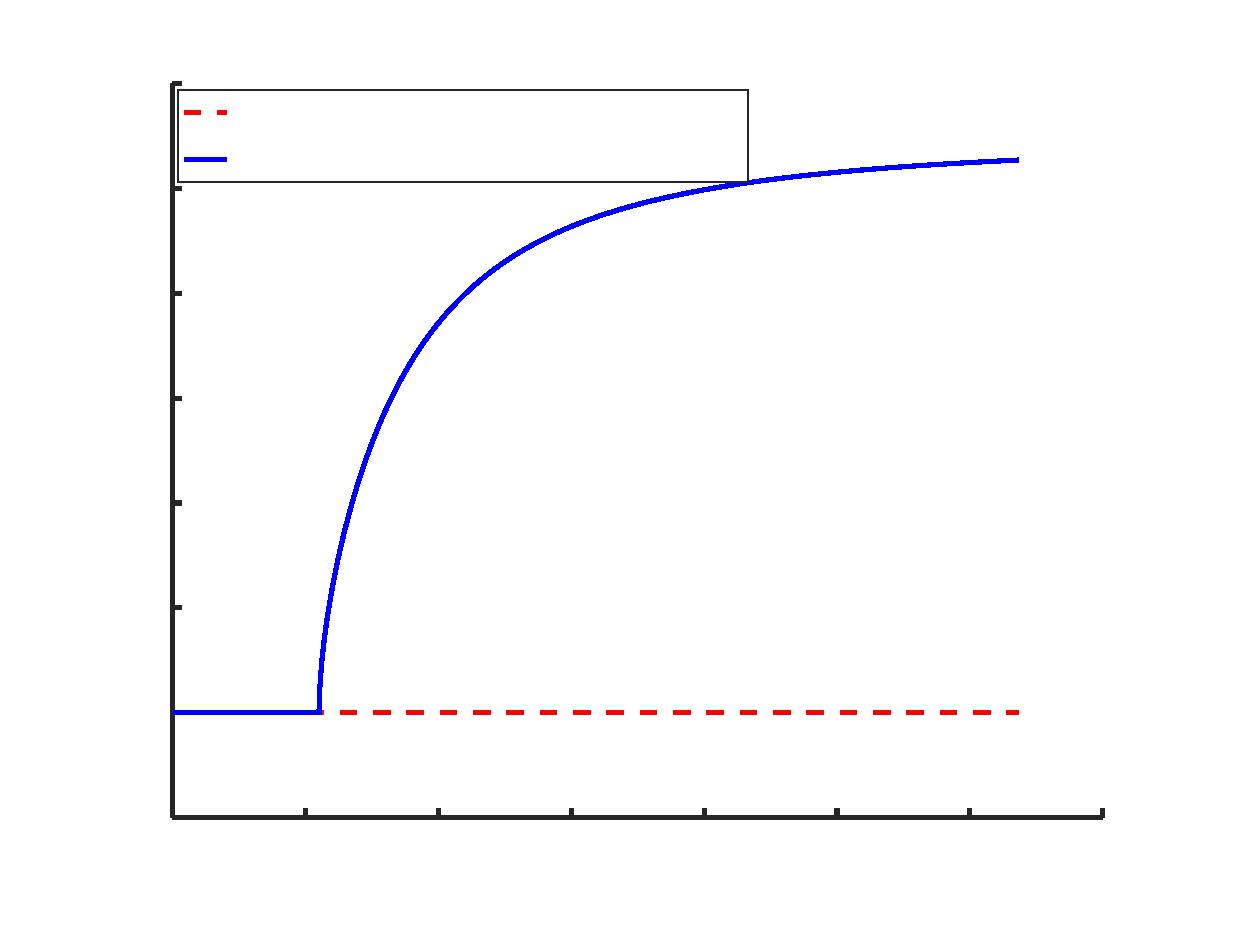
\includegraphics{stabNewmark-inc}
\end{picture}%
\begin{picture}(576,432)(0,0)
\fontsize{16}{0}
\selectfont\put(74.88,42.5189){\makebox(0,0)[t]{\textcolor[rgb]{0.15,0.15,0.15}{{0}}}}
\fontsize{16}{0}
\selectfont\put(138.651,42.5189){\makebox(0,0)[t]{\textcolor[rgb]{0.15,0.15,0.15}{{0.5}}}}
\fontsize{16}{0}
\selectfont\put(202.423,42.5189){\makebox(0,0)[t]{\textcolor[rgb]{0.15,0.15,0.15}{{1}}}}
\fontsize{16}{0}
\selectfont\put(266.194,42.5189){\makebox(0,0)[t]{\textcolor[rgb]{0.15,0.15,0.15}{{1.5}}}}
\fontsize{16}{0}
\selectfont\put(329.966,42.5189){\makebox(0,0)[t]{\textcolor[rgb]{0.15,0.15,0.15}{{2}}}}
\fontsize{16}{0}
\selectfont\put(393.737,42.5189){\makebox(0,0)[t]{\textcolor[rgb]{0.15,0.15,0.15}{{2.5}}}}
\fontsize{16}{0}
\selectfont\put(457.509,42.5189){\makebox(0,0)[t]{\textcolor[rgb]{0.15,0.15,0.15}{{3}}}}
\fontsize{16}{0}
\selectfont\put(521.28,42.5189){\makebox(0,0)[t]{\textcolor[rgb]{0.15,0.15,0.15}{{3.5}}}}
\fontsize{16}{0}
\selectfont\put(69.8755,47.52){\makebox(0,0)[r]{\textcolor[rgb]{0.15,0.15,0.15}{{0.5}}}}
\fontsize{16}{0}
\selectfont\put(69.8755,97.8171){\makebox(0,0)[r]{\textcolor[rgb]{0.15,0.15,0.15}{{1}}}}
\fontsize{16}{0}
\selectfont\put(69.8755,148.114){\makebox(0,0)[r]{\textcolor[rgb]{0.15,0.15,0.15}{{1.5}}}}
\fontsize{16}{0}
\selectfont\put(69.8755,198.411){\makebox(0,0)[r]{\textcolor[rgb]{0.15,0.15,0.15}{{2}}}}
\fontsize{16}{0}
\selectfont\put(69.8755,248.709){\makebox(0,0)[r]{\textcolor[rgb]{0.15,0.15,0.15}{{2.5}}}}
\fontsize{16}{0}
\selectfont\put(69.8755,299.006){\makebox(0,0)[r]{\textcolor[rgb]{0.15,0.15,0.15}{{3}}}}
\fontsize{16}{0}
\selectfont\put(69.8755,349.303){\makebox(0,0)[r]{\textcolor[rgb]{0.15,0.15,0.15}{{3.5}}}}
\fontsize{16}{0}
\selectfont\put(69.8755,399.6){\makebox(0,0)[r]{\textcolor[rgb]{0.15,0.15,0.15}{{4}}}}
\fontsize{16}{0}
\selectfont\put(298.08,23.5189){\makebox(0,0)[t]{\textcolor[rgb]{0.15,0.15,0.15}{{$\Delta t / T$}}}}
\fontsize{16}{0}
\selectfont\put(40.8755,223.56){\rotatebox{90}{\makebox(0,0)[b]{\textcolor[rgb]{0.15,0.15,0.15}{{$\rho(A)$}}}}}
\fontsize{16}{0}
\selectfont\put(103.682,385.714){\makebox(0,0)[l]{\textcolor[rgb]{0,0,0}{{Trapecio: $\alpha=1/4$, $\beta=1/2$}}}}
\fontsize{16}{0}
\selectfont\put(103.682,363.428){\makebox(0,0)[l]{\textcolor[rgb]{0,0,0}{{Acc.Lineal: $\alpha=1/6$, $\beta=1/2$}}}}
\end{picture}
}
	\caption{Estabilidad de variantes del Método de Newmark (Trapecio y Acel. Lineal).}
	\label{fig:stabnewmark}
\end{figure}

Se puede observar que el Método del Trapecio es incondicionalmente estable, mientras que el método de aceleración lineal es condicionalmente estable.

\subsubsection{Ejemplo - Edificio bajo Acción Sísmica}

Finalmente, se presenta un ejemplo en el cual se realiza el análisis dinámico lineal del edificio definido en la Sección~\ref{EjBlast} bajo una acción sísmica. %
%
Para analizar el edificio sometido a movimientos sísmicos laterales de su base, es necesario definir coordenadas absolutas para expresar el movimiento del suelo y otras coordenadas relativas al referencial solidario al suelo.

Los desplazamientos absolutos serán: $\bfu_{G,t}=x_{S,t}\boldsymbol{\iota} + \bfu_{t}$. Donde $\bfu_{G,t}$ son desplazamientos absolutos, $x_{S,t}\boldsymbol{\iota}$ indica la posición del suelo respecto del referencial absoluto y $\bfu_t$ son desplazamientos del edificio relativos al referencial solidario al suelo. Notar que el vector: $\boldsymbol{\iota}$, llamado vector de influencia, indica cómo influye el movimiento de suelo en cada uno de los grados de libertad de la estructura.

Derivando dos veces respecto del tiempo se obtiene: $\ddot{\bfu}_{G,t}=\ddot{x}_{S,t}\boldsymbol{\iota} + \ddot{\bfu}_{t}$. 

Finalmente, notando que las fuerzas internas y los efectos disipativos de la estructura dependen de los desplazamientos relativos $\bfu_t$ y de su derivada primera $\dot{\bfu}_t$, se llega a la ecuación de movimiento bajo acción sísmica:
%
\begin{equation}\label{EcMovLinSismo}
\bfM \ddot{\bfu}_t + \bfC \dot{\bfu}_t + \bfK \bfu_t = -\ddot{x}_{G,t}\bfM \boldsymbol{\iota},
\end{equation}
%
donde $\ddot{x}_{G,t}$ tiene el registro de aceleraciones de suelo medidos según una dirección dada.

En el presente ejemplo, los datos de aceleración corresponden al sismo de Loma Prieta, ocurrido el 17 de octubre de 1987 en California, U.S.A. %\footnote{Obtenidos de \url{http://peer.berkeley.edu/products/strong_ground_motion_db.html}} 

En la Figura~\ref{fig:LomaPrieta} se muestran los resultados de la solución de la dinámica del edificio para la aceleración de terreno elegida. %
Comparando los resultados obtenidos con los de la solución de la dinámica del edificio sometido a una detonación, se observa mayores desplazamientos en el caso del sismo.

\begin{figure}[htb]
	\centering
	\resizebox{.95\linewidth}{!}{% Title: gl2ps_renderer figure
% Creator: GL2PS 1.4.0, (C) 1999-2017 C. Geuzaine
% For: Octave
% CreationDate: Fri Dec 29 11:53:58 2017
\setlength{\unitlength}{1pt}
\begin{picture}(0,0)
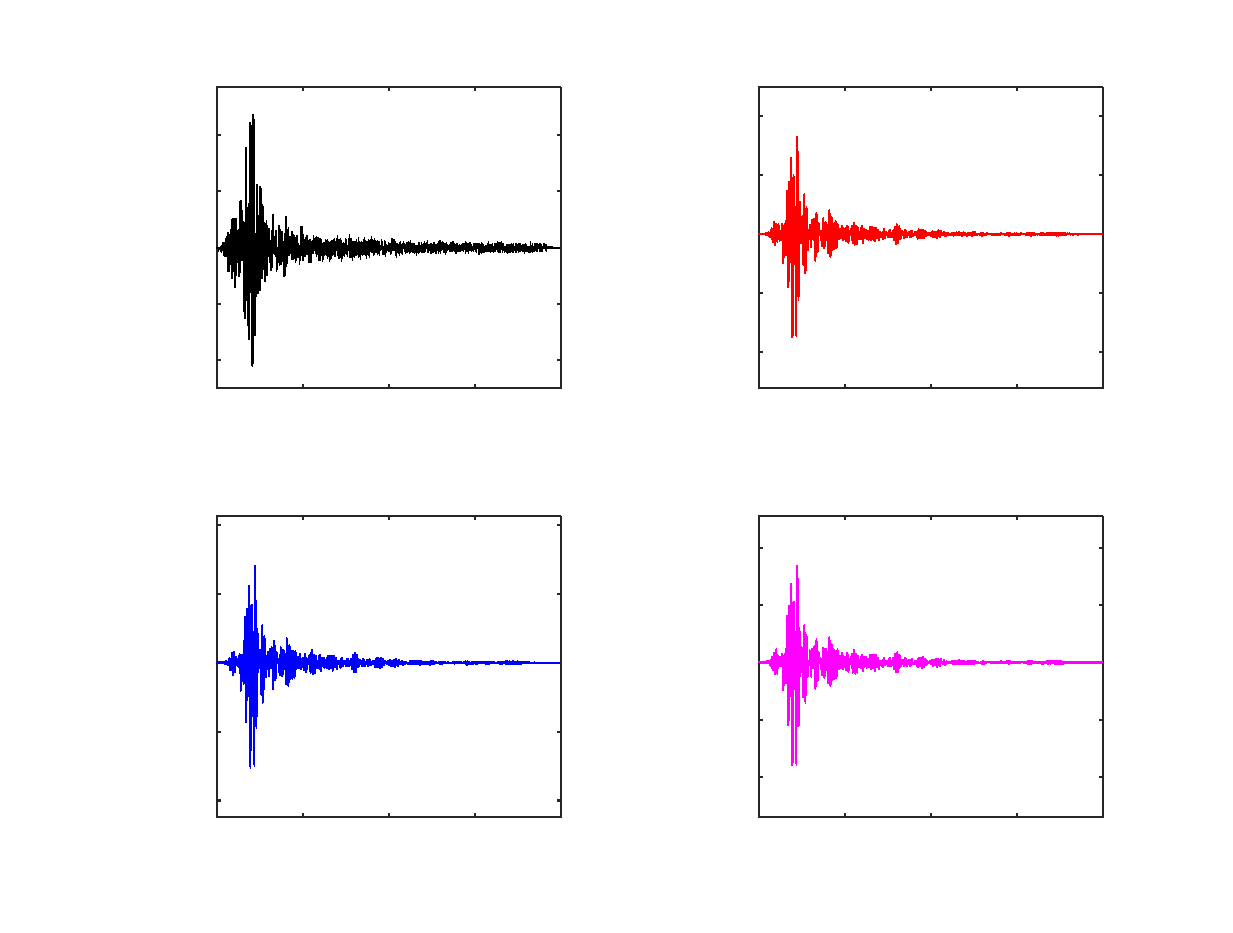
\includegraphics{sismo-inc}
\end{picture}%
\begin{picture}(576,432)(0,0)
\fontsize{15}{0}
\selectfont\put(356.265,248.393){\makebox(0,0)[t]{\textcolor[rgb]{0.15,0.15,0.15}{{0}}}}
\fontsize{15}{0}
\selectfont\put(397.519,248.393){\makebox(0,0)[t]{\textcolor[rgb]{0.15,0.15,0.15}{{10}}}}
\fontsize{15}{0}
\selectfont\put(438.773,248.393){\makebox(0,0)[t]{\textcolor[rgb]{0.15,0.15,0.15}{{20}}}}
\fontsize{15}{0}
\selectfont\put(480.026,248.393){\makebox(0,0)[t]{\textcolor[rgb]{0.15,0.15,0.15}{{30}}}}
\fontsize{15}{0}
\selectfont\put(521.28,248.393){\makebox(0,0)[t]{\textcolor[rgb]{0.15,0.15,0.15}{{40}}}}
\fontsize{15}{0}
\selectfont\put(351.265,270.871){\makebox(0,0)[r]{\textcolor[rgb]{0.15,0.15,0.15}{{-0.01}}}}
\fontsize{15}{0}
\selectfont\put(351.265,299.164){\makebox(0,0)[r]{\textcolor[rgb]{0.15,0.15,0.15}{{-0.005}}}}
\fontsize{15}{0}
\selectfont\put(351.265,327.457){\makebox(0,0)[r]{\textcolor[rgb]{0.15,0.15,0.15}{{0}}}}
\fontsize{15}{0}
\selectfont\put(351.265,355.75){\makebox(0,0)[r]{\textcolor[rgb]{0.15,0.15,0.15}{{0.005}}}}
\fontsize{15}{0}
\selectfont\put(351.265,384.042){\makebox(0,0)[r]{\textcolor[rgb]{0.15,0.15,0.15}{{0.01}}}}
\fontsize{15}{0}
\selectfont\put(438.773,230.393){\makebox(0,0)[t]{\textcolor[rgb]{0.15,0.15,0.15}{{t [s]}}}}
\fontsize{15}{0}
\selectfont\put(297.265,325.629){\rotatebox{90}{\makebox(0,0)[b]{\textcolor[rgb]{0.15,0.15,0.15}{{$u_1(t)$ [m]}}}}}
\fontsize{15}{0}
\selectfont\put(96.036,42.5047){\makebox(0,0)[t]{\textcolor[rgb]{0.15,0.15,0.15}{{0}}}}
\fontsize{15}{0}
\selectfont\put(137.29,42.5047){\makebox(0,0)[t]{\textcolor[rgb]{0.15,0.15,0.15}{{10}}}}
\fontsize{15}{0}
\selectfont\put(178.543,42.5047){\makebox(0,0)[t]{\textcolor[rgb]{0.15,0.15,0.15}{{20}}}}
\fontsize{15}{0}
\selectfont\put(219.797,42.5047){\makebox(0,0)[t]{\textcolor[rgb]{0.15,0.15,0.15}{{30}}}}
\fontsize{15}{0}
\selectfont\put(261.051,42.5047){\makebox(0,0)[t]{\textcolor[rgb]{0.15,0.15,0.15}{{40}}}}
\fontsize{15}{0}
\selectfont\put(91.0356,55.6037){\makebox(0,0)[r]{\textcolor[rgb]{0.15,0.15,0.15}{{-0.02}}}}
\fontsize{15}{0}
\selectfont\put(91.0356,88.6513){\makebox(0,0)[r]{\textcolor[rgb]{0.15,0.15,0.15}{{-0.01}}}}
\fontsize{15}{0}
\selectfont\put(91.0356,121.699){\makebox(0,0)[r]{\textcolor[rgb]{0.15,0.15,0.15}{{0}}}}
\fontsize{15}{0}
\selectfont\put(91.0356,154.747){\makebox(0,0)[r]{\textcolor[rgb]{0.15,0.15,0.15}{{0.01}}}}
\fontsize{15}{0}
\selectfont\put(91.0356,187.794){\makebox(0,0)[r]{\textcolor[rgb]{0.15,0.15,0.15}{{0.02}}}}
\fontsize{15}{0}
\selectfont\put(178.543,24.5047){\makebox(0,0)[t]{\textcolor[rgb]{0.15,0.15,0.15}{{t [s]}}}}
\fontsize{15}{0}
\selectfont\put(47.0355,119.74){\rotatebox{90}{\makebox(0,0)[b]{\textcolor[rgb]{0.15,0.15,0.15}{{$u_2(t)$ [m]}}}}}
\fontsize{15}{0}
\selectfont\put(356.265,42.5047){\makebox(0,0)[t]{\textcolor[rgb]{0.15,0.15,0.15}{{0}}}}
\fontsize{15}{0}
\selectfont\put(397.519,42.5047){\makebox(0,0)[t]{\textcolor[rgb]{0.15,0.15,0.15}{{10}}}}
\fontsize{15}{0}
\selectfont\put(438.773,42.5047){\makebox(0,0)[t]{\textcolor[rgb]{0.15,0.15,0.15}{{20}}}}
\fontsize{15}{0}
\selectfont\put(480.026,42.5047){\makebox(0,0)[t]{\textcolor[rgb]{0.15,0.15,0.15}{{30}}}}
\fontsize{15}{0}
\selectfont\put(521.28,42.5047){\makebox(0,0)[t]{\textcolor[rgb]{0.15,0.15,0.15}{{40}}}}
\fontsize{15}{0}
\selectfont\put(351.265,66.824){\makebox(0,0)[r]{\textcolor[rgb]{0.15,0.15,0.15}{{-0.02}}}}
\fontsize{15}{0}
\selectfont\put(351.265,94.3379){\makebox(0,0)[r]{\textcolor[rgb]{0.15,0.15,0.15}{{-0.01}}}}
\fontsize{15}{0}
\selectfont\put(351.265,121.852){\makebox(0,0)[r]{\textcolor[rgb]{0.15,0.15,0.15}{{0}}}}
\fontsize{15}{0}
\selectfont\put(351.265,149.366){\makebox(0,0)[r]{\textcolor[rgb]{0.15,0.15,0.15}{{0.01}}}}
\fontsize{15}{0}
\selectfont\put(351.265,176.88){\makebox(0,0)[r]{\textcolor[rgb]{0.15,0.15,0.15}{{0.02}}}}
\fontsize{15}{0}
\selectfont\put(438.773,24.5047){\makebox(0,0)[t]{\textcolor[rgb]{0.15,0.15,0.15}{{t [s]}}}}
\fontsize{15}{0}
\selectfont\put(307.265,119.74){\rotatebox{90}{\makebox(0,0)[b]{\textcolor[rgb]{0.15,0.15,0.15}{{$u_3(t)$ [m]}}}}}
\fontsize{15}{0}
\selectfont\put(96.036,248.393){\makebox(0,0)[t]{\textcolor[rgb]{0.15,0.15,0.15}{{0}}}}
\fontsize{15}{0}
\selectfont\put(137.29,248.393){\makebox(0,0)[t]{\textcolor[rgb]{0.15,0.15,0.15}{{10}}}}
\fontsize{15}{0}
\selectfont\put(178.543,248.393){\makebox(0,0)[t]{\textcolor[rgb]{0.15,0.15,0.15}{{20}}}}
\fontsize{15}{0}
\selectfont\put(219.797,248.393){\makebox(0,0)[t]{\textcolor[rgb]{0.15,0.15,0.15}{{30}}}}
\fontsize{15}{0}
\selectfont\put(261.051,248.393){\makebox(0,0)[t]{\textcolor[rgb]{0.15,0.15,0.15}{{40}}}}
\fontsize{15}{0}
\selectfont\put(91.0356,266.84){\makebox(0,0)[r]{\textcolor[rgb]{0.15,0.15,0.15}{{-0.4}}}}
\fontsize{15}{0}
\selectfont\put(91.0356,293.919){\makebox(0,0)[r]{\textcolor[rgb]{0.15,0.15,0.15}{{-0.2}}}}
\fontsize{15}{0}
\selectfont\put(91.0356,320.998){\makebox(0,0)[r]{\textcolor[rgb]{0.15,0.15,0.15}{{0}}}}
\fontsize{15}{0}
\selectfont\put(91.0356,348.077){\makebox(0,0)[r]{\textcolor[rgb]{0.15,0.15,0.15}{{0.2}}}}
\fontsize{15}{0}
\selectfont\put(91.0356,375.156){\makebox(0,0)[r]{\textcolor[rgb]{0.15,0.15,0.15}{{0.4}}}}
\fontsize{15}{0}
\selectfont\put(178.543,230.393){\makebox(0,0)[t]{\textcolor[rgb]{0.15,0.15,0.15}{{t [s]}}}}
\fontsize{15}{0}
\selectfont\put(57.0355,325.629){\rotatebox{90}{\makebox(0,0)[b]{\textcolor[rgb]{0.15,0.15,0.15}{{accel [g]}}}}}
\fontsize{11}{0}
\selectfont\put(178.543,407.849){\makebox(0,0)[b]{\textcolor[rgb]{0,0,0}{{Aceleracion del Terreno por Sismo}}}}
\end{picture}
}
	\caption{Solución numérica del movimiento del edificio bajo acción de sismo.}
	\label{fig:LomaPrieta}
\end{figure}


\section{Dinámica No Lineal}\label{DinNoLin}

Luego de haber estudiado los procedimientos de solución de la ecuación de movimiento para una estructura sin considerar no linealidades, se puede pasar a estudiar los cambios necesarios para poder resolver la dinámica considerando no linealidades, es decir Dinámica No Lineal.

Tal como fue presentada en la Sección \ref{EcMov}, la ecuación de movimiento para una estructura no lineal tiene un vector de fuerzas internas que es función de $\bfu_t$. Dicho vector puede contemplar no linealidad material, geométrica o de ambos tipos.
%
\begin{equation}
\bfM \ddot{\bfu}_t + \bfC \dot{\bfu}_t + \bff_{\text{int}}(\bfu_t) = \bff_{\text{ext},t}
\end{equation}

Los procedimientos de solución explícitos e implícitos se deben ajustar al hecho de que el vector de fuerzas internas ya no es simplemente el producto de la matriz de rigidez por el vector de desplazamientos en el tiempo considerado. %
%
Este cambio tiene un efecto menor en el procedimiento correspondiente al Método de Diferencia Centrada, pero implica un cambio significativo en el procedimiento asociado al Método de Newmark.

De manera resumida, en el caso de dinámica no lineal, se deberá asegurar que el equilibrio se verifica para cada instante de tiempo. En el caso de métodos explícitos eso es inmediato, pero en el caso de métodos implícitos esto requerirá de iteraciones de tipo N-R para asegurar dicho equilibrio.

También cabe mencionar que los criterios de estabilidad numérica vistos para el caso de estructuras lineales no aplican de manera inmediata al caso no lineal. En particular, siempre y cuando el paso temporal ($\Delta t$) sea suficientemente corto, tal que la estructura mantenga un comportamiento aproximadamente lineal durante varios instantes de tiempo, los criterios de estabilidad tendrán cierto grado de validez. Se debe tomar en cuenta que los períodos de vibración relevantes para determinar la estabilidad numérica corresponden a la rigidez de la estructura a medida que transcurre el tiempo. Una estructura que se vuelve más rígida por efectos geométricos a medida que avanza el tiempo, tendrá, para el Método de Diferencia Centrada, un paso temporal crítico cada vez menor debido a dicho aumento de la rigidez.

Para pasos temporales largos, tales que de un instante a otro el comportamiento de la estructura no puede considerarse aproximadamente lineal, los criterios de estabilidad no aplican y se pueden llegar a observar inestabilidades numéricas en métodos que se clasificaron como incondicionalmente estables para problemas lineales.

\subsection{Método de Diferencia Centrada - Explícito}

La deducción del método es idéntica a la presentada en la sección de dinámica lineal. Se busca determinar $\bfu_{t+\Delta t}$, para ello se considera el equilibrio dinámico en el tiempo $t$ y se usan los mismos cocientes incrementales para aproximar las derivadas primera y segunda de $\bfu_t$. En este caso se debe simplemente tomar en cuenta que las fuerzas internas están dadas por $\bff_{\text{int}}(\bfu_{t})$.

Usando la Ecuación~\eqref{EcDifCent} se puede escribir,
%
\begin{equation}\label{EcDifCentNL}
\begin{split}
\left[\frac{1}{\Delta t^2}\bfM + \frac{1}{2\Delta t}\bfC \right] \bfu_{t+\Delta t} = \bff_{ext,t} - &\bff_{\text{int}}(\bfu_{t}) + \frac{2}{\Delta t ^2}\bfM \bfu_t \\
- & \left[\frac{1}{\Delta t^2}\bfM-\frac{1}{2\Delta t}\bfC\right] \bfu_{t-\Delta t}.
\end{split}
\end{equation}

La Ecuación~\eqref{EcDifCentNL} provee la regla mediante la cual se calcula $\bfu_{t+\Delta t}$. Notar que en el caso de una estructura no lineal debemos en cada paso evaluar el vector de fuerzas internas en el instante de tiempo actual. Es claro que el método continúa siendo explícito. 

Se destaca que sigue siendo necesario, tal como en la solución de problemas lineales, que la matriz de masa y eventualmente la de amortiguamiento sean diagonales de manera que la evaluación de $\bfu_{t+\Delta t}$ a partir de la Ecuación~\eqref{EcDifCentNL} sea computacionalmente económica.

A partir del desarrollo anterior, se puede actualizar el procedimiento de solución del Método de Diferencia Centrada para el caso de estructuras no lineales tal como se muestra en el Algoritmo~\ref{PCDifCentNL}.

\begin{algorithm}
	
	\caption{Método de Diferencia Centrada - No-Lineal}
	\label{PCDifCentNL}
	
	\begin{algorithmic}[1]
		
		\STATE Ensamblar: $\bfM$ y $\bfC$ a nivel de estructura.
		\STATE Definir: tiempo final de análisis dinámico: $t_f$
		\STATE Definir: Condiciones iniciales: $\bfu_{0}$, $\dot{\bfu}_{0}$
		\STATE Calcular: $\ddot{\bfu}_{0}\leftarrow \bfM^{-1}(\bff_{ext,t} - \bfC \dot{\bfu}_0 - \bff_{\text{int}}(\bfu_0))$
		\STATE Definir: $\Delta t$, considerar estabilidad numérica.
		\STATE Calcular: $a_0\leftarrow1/\Delta t^2$, $a_1\leftarrow1/(2\Delta t)$, $a_2\leftarrow2a_0$ y $a_3\leftarrow1/a_2$
		\STATE Calcular: $\bfu_{-\Delta t} \leftarrow \bfu_0 - \Delta t \dot{\bfu}_0 + a_3\ddot{\bfu}_0$
		\STATE Calcular y factorizar: $\hat{\bfM}\leftarrow a_0\bfM+a_1\bfC$
		\STATE $t \leftarrow 0$
		\WHILE{$t<t_f$}
		\STATE Calcular: $\hat{\bff}_t\leftarrow \bff_{ext,t} -\bff_{\text{int}}(\bfu_t) +a_2\bfM \bfu_t - (a_0\bfM-a_1\bfC)\bfu_{t-\Delta t}$
		\STATE Resolver: $\bfu_{t+\Delta t}\leftarrow \hat{\bfM}^{-1}\hat{\bff}_t$
		\STATE Calcular aceleración: $\ddot{\bfu}_{t}\leftarrow a_0(\bfu_{t+\Delta t}-2\bfu_{t}+\bfu_{t-\Delta t})$
		\STATE Calcular velocidad: $\dot{\bfu}_{t}\leftarrow a_1(\bfu_{t+\Delta t}-\bfu_{t-\Delta t})$
		\STATE $t\leftarrow t+\Delta t$
		\ENDWHILE
		
	\end{algorithmic}
	
\end{algorithm}

En este momento es una buena idea comentar sobre la elección del paso temporal ($\Delta t$) para el Método de Diferencia Centrada en problemas no lineales. Tal como se mencionó anteriormente, la estabilidad numérica del método continúa restringiendo el paso temporal máximo que se puede usar. La elección del paso se vuelve más difícil en el caso de estructuras no lineales ya que el paso temporal crítico no es constante durante la solución. %
%
La rigidez de la estructura puede variar a lo largo del tiempo por efectos de rigidez geométrica o por no linealidad material. Si se espera que la estructura solamente se flexibilice a medida que transcurre el tiempo, un criterio razonable puede ser determinar el paso temporal en base a la rigidez inicial de la estructura. Si este no es el caso, se debe prever el efecto de la rigidización de la estructura en el paso temporal crítico y asegurar que el paso elegido no superará el valor crítico mínimo previsto.

Al realizar análisis dinámicos de estructuras no lineales usando el Método de Diferencia centrada, la elección de un paso temporal demasiado largo en comparación con el mínimo paso temporal crítico previsto, puede llevar a acumular errores significativos durante aquellos instantes de tiempo en los cuales el paso temporal elegido superó al paso crítico. %
%
Esta acumulación acotada de errores es marcadamente distinta a la que se observa en análisis dinámicos lineales, en los cuales si se elije un paso temporal por encima del valor crítico, la solución diverge y el analista puede reconocer fácilmente que seleccionó un paso temporal erróneo.


\subsubsection{Ejemplo Dinámica No Lineal - Cercha de Von Mises}

Se considera una cercha de tipo de Von Mises bajo la acción de una carga dinámica. %
%
La estructura consiste en dos columnas flexibles empotradas en la base y dos bielas articuladas que trabajan como puntales de la cercha tal como se muestra en la Figura~\ref{fig:GeomVM}. %

Se coloca una masa $m$ suspendida de la cumbre de la cercha. %
%
Todas las barras de la cercha están formada por acero ($E=200 \text{ GPa}$) y sección rectangular ($a=3.2\text{mm}$ y $b=25.4\text{mm}$). %
%
Los parámetros que definen la geometría son: $L_c = 240 $ mm, $L_x= 187$ mm y $L_z=84$ mm. %
%
Esta estructura es la utilizada por el profesor A. Wadee en la presentación referida al inicio del Capítulo 2 de este documento.

\begin{figure}[htb]
	\centering
	\def\svgwidth{0.7\textwidth}
\input{../fig/misses_truss_Cap4.pdf_tex}
	\caption{Geometría de Cercha de Von Mises.}
	\label{fig:GeomVM}
\end{figure}

La forma de cargar la estructura consiste en suspender la masa en la configuración indeformada y luego dejarla libre. Esto implica que el vector de deformación inicial es nulo y también lo es el vector de velocidades inicial.

Dada la simetría axial, respecto al eje vertical, presente en la estructura y las cargas aplicadas, se modela la mitad izquierda de la estructura. %
%
De esta forma solo se debe analizar una biela de Green con condición de borde deslizante vertical en el extremo derecho y deslizante horizontal con resorte en el extremo izquierdo tal como se muestra en la Figura~\ref{fig:ModelVM}. %
%
La constante elástica del resorte está dado por la rigidez flexional de los pilares.

\begin{figure}[htb]
	\centering
	\def\svgwidth{0.6\textwidth}
\input{../fig/misses_truss_Cap4_simetr.pdf_tex}
	\caption{Modelo de Cálculo de Cercha de Von Mises.}
	\label{fig:ModelVM}
\end{figure}

El vector de desplazamientos es considerado $\bfu_t = (u_{1,t}, u_{2,t})^\text{T}$ y por lo tanto la ecuación dinámica está dada por:
%
\begin{equation}
\bfM \ddot{\bfu}_t + \bfC \dot{\bfu}_t + \bff_{\text{int}}(\bfu_t)=\bff_{ext,t}.
\end{equation}	
%
Dado que se está analizando media estructura la matriz de masa es igual a:
%
$$\bfM = \left[\begin{array}{cc}m_b& 0\\ 0& (m_b+m)/2\end{array}\right],$$
%
donde $m_b$ es la masa de una biela o columna y $m$ es la masa suspendida del centro de la cercha. Dicha masa se considera rígidamente vinculada a la cercha en la dirección vertical.

Se considera que existe amortiguamiento, para lo cual se introduce una constante $c$ empírica de amortiguamiento de manera de reproducir un amortiguamiento realista de la estructura. %
%
Se usa $c$ para el grado de libertad de movimiento vertical y $c/10$ para el de movimiento horizontal, por lo que la matriz $\bfC$ está dada por:
$$\bfC = \left[\begin{array}{cc}c/10& 0\\ 0& c\end{array}\right].$$
%
A través de estos amortiguamientos se pretende introducir el arrastre de la pesa debido al aire y la fricción existente en las bisagras que forman las articulaciones de la cercha en el modelo.

Para resolver la dinámica de esta estructura se aplica el Método de Diferencia Centrada, el cual requiere que el usuario calcule únicamente el vector de fuerzas internas. %
%
En lo que sigue se deducirá $\bff_{\text{int}}(\bfu_t)$ asumiendo que las bielas son de tipo Green y que la columna se puede modelar como un resorte lineal horizontal de constante $k_c$,  donde $k_c$ está dado por la rigidez flexional $3 E I_c / L_c^3$.

El vector de fuerzas internas de la biela se deduce usando el PTV. Evaluando el trabajo virtual interno se tiene:
%
\begin{equation}
\delta W_{\text{int}}=\delta\bfu^T \bff_{\text{int}}(\bfu_t)= \int_{l_0} \sigma_t \delta\varepsilon_G A dx + \delta\bfu^T\bfK_s \bfu_t,
\end{equation}
%
donde el segundo sumando del trabajo virtual interno corresponde al trabajo virtual interno de la fuerza realizada por el resorte horizontal de constante $k_c$.

La deformación unitaria de Green para la biela está dada por:
%
\begin{equation}
\varepsilon_G = \frac{l_t^2 - l_0^2}{2 l_0^2}.
\end{equation}

Se asume una relación constitutiva elástica lineal entre tensión y deformación de Green, válido para pequeñas deformaciones unitarias pero grandes desplazamientos y rotaciones.
%
\begin{equation}
\sigma = E \varepsilon_G.
\end{equation}

Los largos de barra iniciales (de referencia) y actuales (deformada) se pueden escribir como:
%
\begin{equation}
l_0 ^2 = L_x^2+ L_z^2 \quad \text{y} \quad 
l_t ^2 = (L_x-u_{1,t})^2+ (L_z+u_{2,t})^2,
\end{equation}
respectivamente, con lo cual la deformación de Green se reduce a:
%
\begin{equation}
\varepsilon_G = \frac{-2 L_x u_{1,t}+2 L_z u_{2,t} + u_{1,t}^2 + u_{2,t}^2}{2 (L_x^2+L_z^2)}.
\end{equation}

Se procede a calcular la variación de la deformación de Green ($\delta \varepsilon_G$):
%
\begin{eqnarray}
	\delta \varepsilon_G &=& \dfrac{1}{L_x^2+L_z^2}\left[ (-L_x + u_1)\delta u_1 + (L_z+u_2)\delta u_2 \right] \\
	 &=& \delta\bfu^T  \left[\begin{array}{c} -L_x + u_{1,t}\\ L_z + u_{2,t}\end{array}\right] \dfrac{1}{l_0^2},
\end{eqnarray}
con lo cual, el vector de fuerzas internas para la barra de Green y el resorte lineal resulta:
%
\begin{equation}
\begin{split}
	\bff_{\text{int}}(\bfu_t) = \dfrac{E A l_0(u_{1,t}^2 + u_{2,t}^2 -2 L_x u_{1,t}+2 L_z u_{2,t})}{2 l_0^4} &\left[\begin{array}{c} -L_x + u_{1,t}\\ L_z + u_{2,t}\end{array}\right] \\ +& \left[\begin{array}{c} k_c u_{1,t}\\ 0\end{array}\right].
\end{split}
\end{equation}

Finalmente, la fuerza externa dinámica aplicada sobre la cercha resulta en un vector $\bff_{\text{ext},t}$ dado por:
%
\begin{equation}
\bff_{\text{ext},t} = \left[\begin{array}{c} 0\\ -g(m_b+m)/2\end{array}\right].
\end{equation}

\textbf{Solución Numérica - Método de Diferencia Centrada:}

Para obtener la solución numérica se debe definir un paso temporal $\Delta t$ tal que el método de Diferencia Centrada sea estable.

\cajaactividad{
Discutir y estimar cuánto vale $\Delta T_{cr}$ para el ejemplo de la cercha de Von Mises.
}

Luego de definido $\Delta T_{cr}$ se procede a implementar el método. En el Código~\ref{cod:VonMisesCod} se muestra una implementación para la resolución del ejemplo.

\lstinputlisting[caption = {Código para análisis dinámico de cercha de Von Mises.}\label{cod:VonMisesCod}]{../src/VonMisesNL_DifCent.m}

En la Figura~\ref{fig:ResVM} se muestra la solución de la dinámica para una masa suspendida igual a $m = 1.4$ kg.

\begin{figure}[!htb]
	\centering
	\resizebox{.95\linewidth}{!}{% Title: gl2ps_renderer figure
% Creator: GL2PS 1.4.0, (C) 1999-2017 C. Geuzaine
% For: Octave
% CreationDate: Fri Dec 29 11:58:15 2017
\setlength{\unitlength}{1pt}
\begin{picture}(0,0)
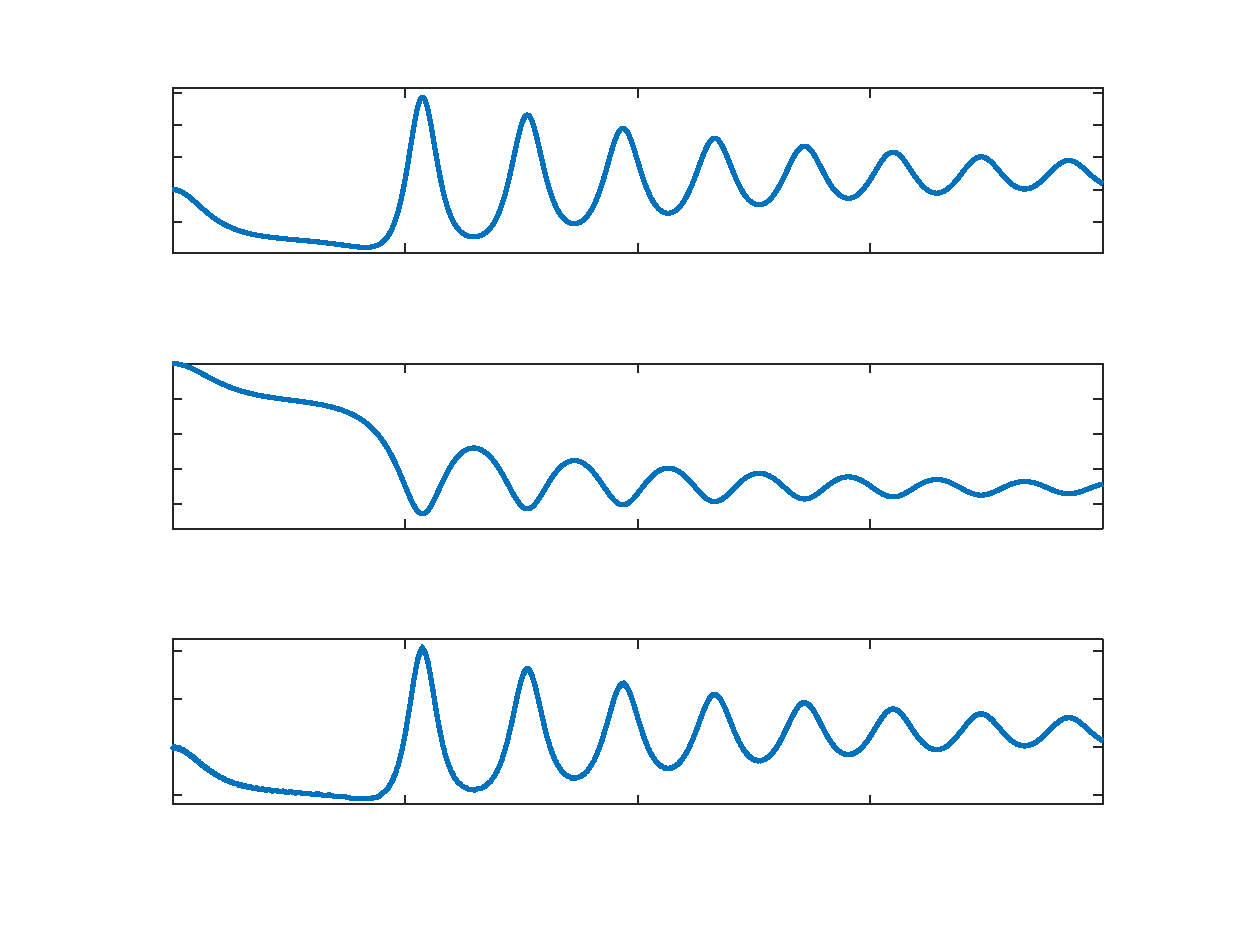
\includegraphics{PlotsVMises-inc}
\end{picture}%
\begin{picture}(576,432)(0,0)
\fontsize{16}{0}
\selectfont\put(74.88,313.318){\makebox(0,0)[t]{\textcolor[rgb]{0.15,0.15,0.15}{{0}}}}
\fontsize{16}{0}
\selectfont\put(186.48,313.318){\makebox(0,0)[t]{\textcolor[rgb]{0.15,0.15,0.15}{{0.5}}}}
\fontsize{16}{0}
\selectfont\put(298.08,313.318){\makebox(0,0)[t]{\textcolor[rgb]{0.15,0.15,0.15}{{1}}}}
\fontsize{16}{0}
\selectfont\put(409.68,313.318){\makebox(0,0)[t]{\textcolor[rgb]{0.15,0.15,0.15}{{1.5}}}}
\fontsize{16}{0}
\selectfont\put(521.28,313.318){\makebox(0,0)[t]{\textcolor[rgb]{0.15,0.15,0.15}{{2}}}}
\fontsize{16}{0}
\selectfont\put(69.8755,333.446){\makebox(0,0)[r]{\textcolor[rgb]{0.15,0.15,0.15}{{-10}}}}
\fontsize{16}{0}
\selectfont\put(69.8755,348.867){\makebox(0,0)[r]{\textcolor[rgb]{0.15,0.15,0.15}{{0}}}}
\fontsize{16}{0}
\selectfont\put(69.8755,364.287){\makebox(0,0)[r]{\textcolor[rgb]{0.15,0.15,0.15}{{10}}}}
\fontsize{16}{0}
\selectfont\put(69.8755,379.707){\makebox(0,0)[r]{\textcolor[rgb]{0.15,0.15,0.15}{{20}}}}
\fontsize{16}{0}
\selectfont\put(69.8755,395.128){\makebox(0,0)[r]{\textcolor[rgb]{0.15,0.15,0.15}{{30}}}}
\fontsize{16}{0}
\selectfont\put(298.08,294.318){\makebox(0,0)[t]{\textcolor[rgb]{0.15,0.15,0.15}{{$t$ [s]}}}}
\fontsize{16}{0}
\selectfont\put(39.8755,357.968){\rotatebox{90}{\makebox(0,0)[b]{\textcolor[rgb]{0.15,0.15,0.15}{{$u_1$ [mm]}}}}}
\fontsize{16}{0}
\selectfont\put(74.88,181.025){\makebox(0,0)[t]{\textcolor[rgb]{0.15,0.15,0.15}{{0}}}}
\fontsize{16}{0}
\selectfont\put(186.48,181.025){\makebox(0,0)[t]{\textcolor[rgb]{0.15,0.15,0.15}{{0.5}}}}
\fontsize{16}{0}
\selectfont\put(298.08,181.025){\makebox(0,0)[t]{\textcolor[rgb]{0.15,0.15,0.15}{{1}}}}
\fontsize{16}{0}
\selectfont\put(409.68,181.025){\makebox(0,0)[t]{\textcolor[rgb]{0.15,0.15,0.15}{{1.5}}}}
\fontsize{16}{0}
\selectfont\put(521.28,181.025){\makebox(0,0)[t]{\textcolor[rgb]{0.15,0.15,0.15}{{2}}}}
\fontsize{16}{0}
\selectfont\put(69.8755,198.054){\makebox(0,0)[r]{\textcolor[rgb]{0.15,0.15,0.15}{{-200}}}}
\fontsize{16}{0}
\selectfont\put(69.8755,214.867){\makebox(0,0)[r]{\textcolor[rgb]{0.15,0.15,0.15}{{-150}}}}
\fontsize{16}{0}
\selectfont\put(69.8755,231.68){\makebox(0,0)[r]{\textcolor[rgb]{0.15,0.15,0.15}{{-100}}}}
\fontsize{16}{0}
\selectfont\put(69.8755,248.494){\makebox(0,0)[r]{\textcolor[rgb]{0.15,0.15,0.15}{{-50}}}}
\fontsize{16}{0}
\selectfont\put(69.8755,265.307){\makebox(0,0)[r]{\textcolor[rgb]{0.15,0.15,0.15}{{0}}}}
\fontsize{16}{0}
\selectfont\put(298.08,162.025){\makebox(0,0)[t]{\textcolor[rgb]{0.15,0.15,0.15}{{$t$ [s]}}}}
\fontsize{16}{0}
\selectfont\put(29.8755,225.674){\rotatebox{90}{\makebox(0,0)[b]{\textcolor[rgb]{0.15,0.15,0.15}{{$u_2$ [mm]}}}}}
\fontsize{16}{0}
\selectfont\put(74.88,48.731){\makebox(0,0)[t]{\textcolor[rgb]{0.15,0.15,0.15}{{0}}}}
\fontsize{16}{0}
\selectfont\put(186.48,48.731){\makebox(0,0)[t]{\textcolor[rgb]{0.15,0.15,0.15}{{0.5}}}}
\fontsize{16}{0}
\selectfont\put(298.08,48.731){\makebox(0,0)[t]{\textcolor[rgb]{0.15,0.15,0.15}{{1}}}}
\fontsize{16}{0}
\selectfont\put(409.68,48.731){\makebox(0,0)[t]{\textcolor[rgb]{0.15,0.15,0.15}{{1.5}}}}
\fontsize{16}{0}
\selectfont\put(521.28,48.731){\makebox(0,0)[t]{\textcolor[rgb]{0.15,0.15,0.15}{{2}}}}
\fontsize{16}{0}
\selectfont\put(69.8755,58.3215){\makebox(0,0)[r]{\textcolor[rgb]{0.15,0.15,0.15}{{-50}}}}
\fontsize{16}{0}
\selectfont\put(69.8755,81.347){\makebox(0,0)[r]{\textcolor[rgb]{0.15,0.15,0.15}{{0}}}}
\fontsize{16}{0}
\selectfont\put(69.8755,104.373){\makebox(0,0)[r]{\textcolor[rgb]{0.15,0.15,0.15}{{50}}}}
\fontsize{16}{0}
\selectfont\put(69.8755,127.398){\makebox(0,0)[r]{\textcolor[rgb]{0.15,0.15,0.15}{{100}}}}
\fontsize{16}{0}
\selectfont\put(298.08,29.731){\makebox(0,0)[t]{\textcolor[rgb]{0.15,0.15,0.15}{{$t$ [s]}}}}
\fontsize{16}{0}
\selectfont\put(35.8755,93.3804){\rotatebox{90}{\makebox(0,0)[b]{\textcolor[rgb]{0.15,0.15,0.15}{{Directa [N]}}}}}
\end{picture}
}
	\caption{Resultados de Cercha de Von Mises (m=1.4kg) - Dinámica}
	\label{fig:ResVM}
\end{figure}


Para valores de masa mayores a $1.4$ kg se observa pandeo tipo \textit{Snap-through} dinámico de la estructura.

\cajaactividad{
Compare este valor con el valor de carga crítica correspondiente a carga cuasi-estática.
}


\subsection{Método de Newmark - Implícito}

La deducción de este método es similar a la presentada en la sección de dinámica lineal. %
%
El objetivo es determinar $\bfu_{t+\Delta t}$, para ello Newmark considera el equilibrio dinámico en el tiempo $t+\Delta t$ y se usan las mismas expresiones de tipo Taylor para aproximar $\bfu_{t+\Delta t}$ y $\dot{\bfu}_{t+\Delta t}$. Se debe notar que las fuerzas internas en el tiempo $t+\Delta t$ están dadas por $\bff_{\text{int}}(\bfu_{t+\Delta t})$.

Lo anterior, en conjunto con las Ecuaciones \eqref{Newmark1} y \eqref{Newmark2}, permiten obtener la expresión:
%
\begin{equation}\label{NewmarkNL1}
\bff_{\text{int}}(\bfu_{t+\Delta t})+\left[ \frac{1}{\alpha \Delta t^2} \bfM + \frac{\delta}{\alpha \Delta t} \bfC \right] \bfu_{t+\Delta t} = \hat{\bff}_{t+\Delta t},
\end{equation}
%
donde la definición de $\hat{\bff}_{t+\Delta t}$ es la misma que la dada en la Sección~\ref{FormNewmarkLin}. %

Se observa por lo tanto que para determinar $\bfu_{t+\Delta t}$ mediante Newmark, para el caso de un problema dinámico no lineal, se debe resolver la ecuación no lineal dada por la Ecuación~\eqref{NewmarkNL1}. %
%
Esto es claramente más laborioso que en el caso de un problema dinámico lineal, en el cual cada paso de Newmark consistía simplemente en resolver un sistema de ecuaciones lineales.

\cajaactividad{
Formular la solución de la ecuación no lineal definida en el paso de Newmark aplicando soluciones iterativas de tipo Newton-Raphson o incluso Newton-Raphson modificado.
}

Para los métodos de tipo Newton-Raphson se debe usar la matriz tangente $\bfK_T = \partial \bff_{\text{int}} / \partial \bfu$, que ya fue presentada en el caso de análisis estáticos. %
%
Para que la solución sea correcta se debe iterar hasta obtener convergencia del equilibrio dinámico en el paso $t+\Delta t$, con lo cual los criterios de convergencia son similares a los ya discutidos anteriormente, aunque usando la ecuación no lineal dada en esta sección.

Tal como se indicó al comienzo de esta sección, si el paso temporal es suficientemente corto como para que la estructura se comporte de forma aproximadamente lineal durante varios instantes de tiempo, entonces Newmark presentará un comportamiento estable. A pesar de esto, es posible seleccionar pasos temporales suficientemente largos como para que los análisis de estabilidad numérica, hechos en la hipótesis de dinámica lineal, pierdan validez y el método presente inestabilidad numérica. %
%
Se puede ver un ejemplo de este tipo de comportamiento en el Capítulo 24 del libro \citep{Crisfield1997}.

